\documentclass[a4paper,11pt]{report}
\usepackage{ulem}
\usepackage{a4wide}
\usepackage[dvipsnames,svgnames]{xcolor}
\usepackage[pdftex]{graphicx}
\title{}
\usepackage[utf8]{inputenc}
\usepackage[hidelinks]{hyperref}
\usepackage{listings}
\usepackage{color}
\usepackage[parfill]{parskip}
\usepackage[T1]{fontenc}
\usepackage{tikz}
\usepackage[lighttt]{lmodern}
\definecolor{light-gray}{gray}{0.95}

\lstset{xleftmargin=1cm,
        xrightmargin=1cm,
        framexleftmargin=5mm,
        framexrightmargin=5mm,
        framextopmargin=5mm,
        framexbottommargin=5mm,
        basicstyle=\ttfamily,
        breaklines=true,
        showstringspaces=false,
        backgroundcolor=\color{light-gray},
        keywordstyle=\bfseries,
        commentstyle=\color{gray}
        } 
\lstset{language=Python}
\setcounter{secnumdepth}{1}
\DeclareFontShape{OT1}{cmtt}{bx}{n}{<5><6><7><8><9><10><10.95><12><14.4><17.28><20.74><24.88>cmttb10}{}

% commands generated by html2latex
\makeatletter
\newenvironment{btHighlight}[1][]
{\begingroup\tikzset{bt@Highlight@par/.style={#1}}\begin{lrbox}{\@tempboxa}}
{\end{lrbox}\bt@HL@box[bt@Highlight@par]{\@tempboxa}\endgroup}

\newcommand\btHL[1][]{%
  \begin{btHighlight}[#1]\bgroup\aftergroup\bt@HL@endenv%
}
\def\bt@HL@endenv{%
  \end{btHighlight}%   
  \egroup
}
\newcommand{\bt@HL@box}[2][]{%
  \tikz[#1]{%
    \pgfpathrectangle{\pgfpoint{1pt}{0pt}}{\pgfpoint{\wd #2}{\ht #2}}%
    \pgfusepath{use as bounding box}%
    \node[anchor=base west, fill=orange!30,outer sep=0pt,inner xsep=1pt, inner ysep=0pt, minimum height=\ht\strutbox+1pt,#1]{\raisebox{1pt}{\strut}\strut\usebox{#2}};
  }%
}
\makeatother

\begin{document}

\begin{titlepage}
\begin{center}
{ \huge \bfseries Introductory Programming in Python } \\[5cm]
{\LARGE Copyright \textsc{Umonya}\\
www.umonya.org }\\[1cm]

Original source thanks to \textsc{James Dominy} \\[0.5cm]
With additional thanks to the following contributors: \\[0.5cm]
\begin{tabular}{r l}
\textsc{Nina Schiff} & \textsc{Rizmari Versfeld}\\
\textsc{Lyndsay Lawrence} & \textsc{Bradley Lawrence}\\
\textsc{Johann van den Berg} & \textsc{Jonathan Hitchcock} \\
\textsc{James Saunders} & \textsc{Kaitlyn Crawford} \\
\textsc{Bruce Merry} & \textsc{Yaseen Humdulay} \\
\textsc{Jason Brownbridge} & \\
\end{tabular}
\vfill


\includegraphics[width=0.15\textwidth]{./cc-logo.jpg}~

\includegraphics[width=0.15\textwidth]{./attribution-by.png}~
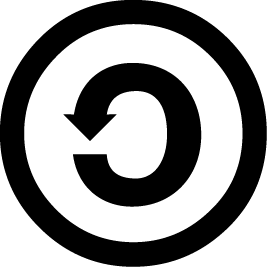
\includegraphics[width=0.15\textwidth]{./share-alike-sa.png}~ \\[0.5cm]
{\large All notes licenced under Creative Commons Attribution-Share-Alike 3.0 } \\
{\large \url{http://creativecommons.org/licenses/by-sa/3.0/deed.en_GB} }\\
\end{center}
\end{titlepage}

\chapter{Basic concepts}
    \section{What is a Program?}

Simply put, a program is a set of instructions on \textbf{how} to    take some \textbf{input} data and produce    \textbf{output} data. Programs can be written in many   languages, such as PERL, Python, C, Ruby, Pascal, etc\ldots\ Even a   stylised form of natural languages such as English, known as pseudo   code, can be used to describe a program effectively.

\begin{center}\textbf{Input -$>$ Program -$>$ Output}\end{center}

It is important to realise that the \textbf{program}   determines what input is satisfactory, and what input will cause error.   Input cannot be used to change how a program works. Similarly, the program   defines what output will be produced. If you need a program to handle   input differently, you need to write a new program. Likewise, if the   output isn't what you need, you will need to change the program too.

Ultimately a program, no matter what language it is written in,   consists of a some atomic actions/instructions, each one an instruction   that cannot be divided into a sequence of 'smaller' or 'less complex'   instructions. These instructions are composed (as in mathematical   composition) in various manners, usually by issuing them in sequential order,   but also by defining the result of one instruction as the operand of   another.

Instructions (or sets of composed instructions) can be divided into   two groups, those that produce a result, and those that   don't. For example, adding two numbers, 3 and 4, together has a result   (7). More specifically, it has a \textbf{value}, i.e. some data   the program can continue to work with. Contrast this with an   instruction that puts a line of text on the screen. It produces no   value as a result. Instructions which produce a value are called   \textbf{expressions}, instructions which produce no value are   called \textbf{statements}

In a similar manner to statements, expressions can be combined with   other expressions, to form complex expressions. Expressions are   combined using \textbf{operators} such as the mathematical   functions sum, difference, product, quotient, etc\ldots\ Thus 1+1 is also   an expression that has \textbf{a single value} despite the fact   that it is a composite of multiple sub-expressions.

Which we can compare to the much simpler version of the same thing   in python
\begin{lstlisting}
a = 12
b = 12
if a*b == 144:
    a = 1
\end{lstlisting}

The basic point is to illustrate that programs are made up of small,   well defined, \textbf{easy to understand} steps in sequence. As   in chess, where each individual piece can only move in a very limited   number of ways, yielding a tiny number of potential moves per piece per   turn, these moves can be combined in a near infinite number of ways and   often grouped together into common techniques or strategies. So too can   the simple statements of a programming language be combined in infinite   ways to produce complex but meaningful results.

\section{Everyone can program!}

Believe it or not, you've programmed before. You've programmed your   friends, and do so every time you give them directions.  After all what   is a set of directions but a sequence of instructions.
\begin{lstlisting}
OUT OF Cape Town TAKE the N1
TAKE the Sable rd. Offramp
AT the fork VEER LEFT
AT the traffic lights TURN LEFT
AT the NEXT traffic lights TURN RIGHT 
AT the traffic circle TURN LEFT
AT the NEXT traffic circle TURN RIGHT 
AT the t-junction TURN LEFT
\end{lstlisting}

You will note that some (in fact a hell of a lot) of the words in   the directions to my place are capitalised. In the language of giving   directions, these are pretty much our most basic instructions. That is, they are the \textbf{atomic} instructions of the program. This means that each of these instructions cannot be divided into a combination of more basic instructions For example, LEFT, on it's own doesn't make sense. Likewise, TURN alone is vague. Thus TURN LEFT would be considered an atomic instruction, which along with other atomic instructions could be used to build up a more complex program of instructions.

The portion   of the directions left in lowercase are labels or names for things that   are not common to all sets of directions, most often places specific to   the set of directions being given. These have values, and would be our   expressions.

Examining the directions we have
\begin{description}
	\item[OUT OF] meaning I must first be \textbf{in} a named place    before performing the next instruction
	\item[TAKE] meaning to drive along, or turn off onto a named offramp
	\item[AT] continue until the named place or situation is reached    \textbf{before} performing the next instruction
	\item[VEER] meaning to stay in a particular lane as the road splits
	\item[TURN LEFT, TURN RIGHT] self explanatory
	\item[NEXT] meaning the next object of specified type encountered
\end{description}

At first the description of these concepts may seem obvious, but   recall that computers, the machines executing your programming   instructions, have an IQ of 0. They are not intelligent, fiendishly   annoying at times perhaps, but never intelligent, never aware, never   capable of the massive amounts of understanding and contextualization done   by the human brain in order to draw logical conclusions. They are designed and built to understand and   execute only specific very basic steps. So what is implicit in the   instructions contained in a set of directions given to us, must be   explicitly defined for a computer.

\section{Data representation and translation of real world problems}

Now that the concept of sequences of statements has been thoroughly   flogged to death, to what do these statements apply? They apply to   \textbf{data}! But data in a computer, like instructions, must   be simple and well defined, or at the very least able to be broken down   into multiple well defined simple pieces. In general computers work   only with numbers. The pictures you see on screen, the text you are   reading, the sound you hear when playing MP3s are all numbers. The   actual physical devices attached to the computer are what are   responsible for transforming the numbers with which the Central Processing Unit, or 'brain' of a computer, deals into   humanly recognisable phenomena such as sound waves and images. Until   the screen, or the speakers, are reached, everything is numbers.  So it   stands to reason that the most basic, atomic, unit of data in a   computer is a number. Fortunately, modern programming languages are   capable of dealing with numbers and sequences of numbers in a few   different ways. Integers and Reals can be considered atomic data units   in almost every modern computer language, as can text in the form of a   string of characters in sequence.

As programs are usually written to solve problems occurring in the   real world, it falls to the programmer to translate the problem being   solved into something the computer can deal with, i.e. numbers. This is   a bit like those annoying word problems we encountered in junior   school mathematics.
\begin{quotation}     Jane has seven apples, Mary has four, Bob has one. They pool their    resources, and divide the apples equally. How many apples does each    one receive?    
\end{quotation}

The most difficult concept to grasp when learning to program is the   ability to translate a problem expressed in words into a set of   instructions that describe the solution to the problem. Learning a   programming language doesn't teach one to program, it merely provides   one with a specific set of tools with which one can solve a problem.   Learning how to apply these tools is the true skill to programming, and   this comes primarily with experience. The problem set out above is   ridiculously simple, and you've already worked out the answer in your   head, but \textbf{how did you do it?} Describe the process! But   what if there were 1000 people involved, and many thousands of apples.   Working it out in your head becomes a tedious task, but the basic   process you followed in your head for three people applies equally well   to the case of a thousand people. And so for our first exercise in   programming let us translate the word problem into the atomic (most basic)   statements and atomic data units that can be used to provide us with   the answer. Assume we are provided with only the following statements   and expressions to work with, and that statements are numbered from 1   upwards in the order in which they appear in our program:
\begin{itemize}
	\item EXPRESSION -- \texttt{input()}: get a number from input
	\item STATEMENT -- \texttt{labelname = \#}: Assign the value of number to    a label for storage
	\item STATEMENT -- \texttt{labelname += \#}: Addition of the second number    to the number stored in labelname
	\item STATEMENT -- \texttt{if \# != \# \{\}}: check if the two numbers    are not equal. If they are not equal perform any instructions    within the braces \texttt{\{\}}
	\item STATEMENT -- \texttt{GOTO \#}: Instead of executing the next    statement, execute the statement numbered \texttt{\#}
	\item STATEMENT -- \texttt{labelname /= \#}: Division of the number stored    in labelname by \texttt{\#}
	\item STATEMENT -- \texttt{print(\#)}: Output of a number to the    screen
\end{itemize}

Note that \texttt{\#} can be either an actual number, the name of a   label storing a number, or the instruction \texttt{input()} which is the   number received as input.
\begin{quotation}     Each of a number of people has at least one apple. They pool their    resources and divide the apples equally. For any given number of    people and the number of apples each of these people has, how many    apples will each person receive?    
\end{quotation}

Given only the above statements and expressions to work with, there   are some important questions that need answering
\begin{itemize}
	\item Do we need to know who started with how many apples?
	\item How do we represent how many apples there are?
	\item How can one determine the total number of people?
\end{itemize}
\begin{lstlisting}
 1: apples = 0
 2: people = 0
 3: a = input()
 4: people += 1
 5: if a != 0 {
 6:     apples += a
 7:     GOTO 3
    }
 8: apples /= people
 9: print(apples)
\end{lstlisting}

\section{Exercises}
\begin{enumerate}
	\item What is a program?
	\item What is the difference between an expression and a    statement?
\end{enumerate}

\chapter{Invocation}
    
\section{Starting the interactive shell}

Starting Python is easy.
\begin{enumerate}
    \item We will be using IDLE to get things started
    \item On the Desktop you will see a link named "Python"
    \item To open the Interpreter click on \textbf{"Run" > "Python Shell"}
    \item The screen will open up and look similar to the following
\end{enumerate}
% <p>Similarly from a terminal in Linux simply type <code>python</code> and press Enter.</p>

\begin{lstlisting}
Python 3.3.0 (v3.3.0:bd8afb90ebf2, Sep 29 2012, 01:25:11) 
[GCC 4.2.1 (Apple Inc. build 5666) (dot 3)] on darwin
Type "copyright", "credits" or "license()" for more information.
>>> WARNING: The version of Tcl/Tk (8.5.9) in use may be unstable.
Visit http://www.python.org/download/mac/tcltk/ for current information.
>>>
\end{lstlisting}

What you see now is known as the Python interactive shell. The first   line tells you what version of Python you are running. The second line   gives you some information about how this particular copy of Python was   built, and on what system it is running. The third line lists some   commands you can use to get more information. Whilst in the interactive   shell, you can enter Python expressions and see their results   immediately. Try it now, type in a simple mathematical expression such   as 
\texttt{4 + 7}.
\begin{lstlisting}
>>> 4 + 7
11
>>>
\end{lstlisting}

As you can see, the answer or result of the expression is printed   out, and you are returned to the prompt \texttt{>>>}. Now try   something different: type in 
\texttt{a = 2 + 7}.  Then, on the   next line, type just 
\texttt{a}.
\begin{lstlisting}
>>> a = 2 + 7
>>> a
9
>>>
\end{lstlisting}

This should be somewhat familiar from the end of the basic concepts   section, where we were assigning a value to a name. In this case the   name is \texttt{a} and the value is the result of \texttt{2 + 7}. Note that no value   is printed out immediately after the assignment. The interactive shell   always prints out the value of expressions, but not of statements. This   means however that the labels to which we assign values, more correctly   called \textbf{variables}, are expressions that evaluate to a   value, which is why it printed out 
\texttt{9} when we input \texttt{a}.

\section{Running a saved Python Script}

Whilst ideal as a calculator and for exploring new ideas quickly, it   would be pretty tedious if we had to re-enter our program into the   interactive shell every time we wanted to run it. So instead we can,   and in fact most often will, save our program code to a file. Program   source code is plain raw text. As such word processors like Microsoft   Word, Wordperfect, Open Office etc\ldots\ are not suitable to the task. We will   look for Idle which is specifically geared towards creating Python programs,   and comes with   Python. 

So now, instead of running the interactive shell, let's write our   first Python program, this is also known as a script. Open up the first window again and do the following
\begin{enumerate}
    \item Click on \textbf{File $>$ Save}
    \item Navigate to /home/\textit{username}/Desktop
    \item Save the file as \textbf{hello.py}
    \item Type the following:
\end{enumerate}
\begin{lstlisting}
print("Hello World!")
\end{lstlisting}

Hit F5, or Click \textbf{Run $>$ Run Module} to    run your program.


\begin{lstlisting}
>>>
Hello World!
>>>
\end{lstlisting}

This is a very simple program, but it should help you get the    idea. The computer is only following the instructions you provided   to it. Lets convert the test we did on the Interpreter to a program.   Save it as \textbf{second.py}.   
\begin{lstlisting}
# My second Python program
# This should add two numbers and output the result
a = 2 + 7
a
\end{lstlisting}

Notice the first and second lines. They contain what are called   \textbf{comments}. Any text following a hash character on a   line in a Python program is a comment, including the hash itself.   Comments are completely ignored by Python, and are there purely to   annotate code and make things easier for humans reading the code. We   use comments to place small reminders within the code for ourselves, or   explain the logic behind particularly tricky sections. As we   progress through the course, you will find the code examples used are   sprinkled more and more liberally with comments explaining how they   work.

Now it would be reasonable to expect that if we ran this program we   would get the same results as given to us by the interactive shell. So,   let's try it.     
\begin{lstlisting}
>>>
>>>
\end{lstlisting}

No output? Nothing? The Python interpreter (python), when called   without a file name following, starts up in the interactive shell. Only   then will it output the results of expressions entered. When invoked   with a file name following, and that file contains Python code, Python   will only produce output if explicitly told to do so. So lets use a trick    from our first program. Modify the code so it looks like the following:
\begin{lstlisting}
#My second Python program
4 + 7 #This should add two numbers and output the result
a = 2 + 7
print(a)
>>>
9
>>>
\end{lstlisting}

Ah, that's better. Again, you should recognise the print statement   from the end of the basic concepts section. The print statement will be   explained in greater detail the next section.

One more important consideration is that Python is \textbf{case   sensitive}. A variable \texttt{a} and another variable \texttt{A} are not the   same, as illustrated below \ldots
\begin{lstlisting}
#This program illustrates how Python is case sensitive

a = 3 # assign a the value 3
A = "Hi" # assign A the value "Hi"

# Check whether assigning to A has changed a
print(a)

# Check that A and a are still different
print("A = ", A, " and  a = ", a)
\end{lstlisting}

Running this produces the output:
\begin{lstlisting}
3
A = Hi  and  a = 3
\end{lstlisting}

\section{Exercises}
\begin{enumerate}
    \item Start the Python interpreter 
    \item Try using the interpreter as a calculator 
    \item Write the Hello World program. 
    \item Write the second program. 
    \item Write a program that prints out your name. 
    \item Consider the following lines of code:
\begin{lstlisting}
a = 9
b = 3
a/b\end{lstlisting}
        \begin{enumerate}
            \item For each of these three lines, which are expressions and     which are statements?
            \item What will the output be if these lines are entered into the     python interactive interpreter?
            \item What will the output be if I run these lines from a     file/script?
            \item What changes need to be made to produce output when I run     these lines from a file/script?
        \end{enumerate}
\end{enumerate}

\chapter{Basic output}
    \section{The print() Statement}

The most basic statement in Python is \texttt{print()}. The \texttt{print()}   statement causes whatever is between the brackets to be outputted to the screen.   We've already encountered it previously, now it's time to understand   how it works. Start up the python interactive shell, and let's explore.   Type the following:
\begin{lstlisting}

>>> print(1)
1
>>> print(173+92)
265
>>> print(173+92.0)
265.0
>>> print("hello")
hello
>>>
\end{lstlisting}

As one can see, the \texttt{print()} statement outputs the   \textbf{value} of the expression immediately following it to   the screen, and moves to the next line. Note that the third print   statement produces slightly different output, namely the extra '.0'.   This is because 92.0 and 92 are different to a computer. 92 is an   integer, whilst 92.0 is a real number, or in computing terms a   \textbf{floating point number} or \textbf{float} for short. The   differences will be covered later.

Also of importance is the expression "hello" (note the double   quotes). The value of "hello" is \textit{hello}, and this is what is   outputted to the screen by the \texttt{print()} statement. \textit{hello} is   designated as a \textbf{string} by enclosing it in quotes. Try   
\texttt{print(hello)} without the quotes and see what happens.
\begin{lstlisting}
>>> print(hello)
Traceback (most recent call last):
  File "<stdin>", line 1, in ?
NameError: name `hello' is not defined
>>>
\end{lstlisting}

What's going on? Welcome to your first bug! We will soon learn to dissect and   understand what all that means, but for the moment it is sufficient to   understand that something has gone wrong. But what? Recall from basic   concepts we were able to store values in \textit{labels} or \textit{variables}.   Python consists of a limited set of key words that have special   meaning. These key words form the list of basic (atomic) statements and   expressions that python knows how to handle. Whenever python encounters   a word is doesn't recognise, it treats this as a label name. It   obviously doesn't recognise 'hello' as a statement, and thus treats it as   a \textbf{variable}. Variables must have a value, because   variables are expressions in and of themselves. But we haven't told   Python what the value of hello is, hence it complains \texttt{'hello' is not defined}.

The \texttt{print()} statement is not so plain and boring as it seems. It can   do a few more things that are worth mentioning. Try entering 
\texttt{print("Jane     has", 7, "apples.")}
\begin{lstlisting}
>>> print("Jane has", 7, "apples")
Jane has 7 apples
>>>
\end{lstlisting}

Of course we could just as easily use 
\texttt{print("Jane has 7   apples")} and get the same result. However, separating the number   7 out illustrates two important things about the \texttt{print()} statement.   Firstly, we can in fact output the values of any number of expressions   in a comma separated list, and secondly the outputs of each of the   expressions in the comma separated list are separated by a single space   each.

Finally, you will notice that the \texttt{print()} statement always ends off   the line, and starts a new one. Simply leaving a comma on the end   prevents this, e.g. 
\texttt{print("Enter your name:",)}. In summary:
\begin{itemize}
	\item The \texttt{print()} statement prints out the \textit{values}  between the     brackets and then prints a new line
	\item An empty \texttt{print()} statement ends the current line and starts a new     one.
	\item The \texttt{print()} statement can print multiple expressions if they are     given in a \textit{comma separated} list. In this case, a space is     included between each expression's outputted value.
	\item The automatic newline outputted by \texttt{print()} can be avoided by     putting a trailing comma in the expression list. This will print a     trailing space instead.
	\item If a \texttt{print()} statement with a trailing comma is followed by an     \textit{empty} \texttt{print()} statement, the trailing space is     suppressed.
\end{itemize}

\section{Some String Basics}

Python treats all text in units called \textbf{strings}. A \textbf{string} is formed   by enclosing some text in quotes. Double quotes, or single quotes may   be used. There is a small limitation to this however, being that a   string cannot be broken across multiple lines.
\begin{lstlisting}
'this is a string of text'
"this is also a string of text"
'this string will
    cause an error, because it spans multiple lines'
\end{lstlisting}

Trying to enter the third string into the interactive shell yields
\begin{lstlisting}
>>> 'this string will
    File "<stdin>", line 1
            'this string will
                            ^
SyntaxError: EOL while scanning single-quoted string
>>>
\end{lstlisting}

EOL meaning End Of Line. If we want to introduce line breaks into   strings we can use two methods. The first, and simplest, is to use   \textit{triple quotes}, meaning three double or three single quotes to indicate   both the beginning and the end of the string, as in
\begin{lstlisting}
>>> """this string will not
...  cause an error
...    just because it is split over three lines"""
'this string will not\n  cause an error\n    just because it is split over three lines'
>>>
\end{lstlisting}

The immediately obvious disadvantage is that everything between the   triple quotes is taken as-is, meaning the second and third lines of my   string which I indented to line up with the beginning of the first line   are indented in the string itself in the form of three spaces after   those \texttt{$\backslash$n} thingies. Speaking of which, what the hell are those things?   Why does our string contain stuff we didn't put there? Well let's try   to print the string out \ldots
\begin{lstlisting}
>>> print("""this string will not
...    cause an error
...    just because it is split over three lines""")
this string will not
   cause an error
   just because it is split over three lines
>>>
\end{lstlisting}

Well the \texttt{$\backslash$n}s are gone, but what were they? Strings are sequences   of characters and are one dimensional. They have no   \textbf{implicit} way to specify a line break, or relative   position, or which characters are where relative to which other   characters in the string in two dimensions, as displayed on a screen.   Hence we get the second method of specifying line breaks within a   string. There are special characters known as \textbf{escape     characters} which mean special things inside strings. They all   start with a backslash \texttt{$\backslash$} which escapes the following character from   the string, or in layman's terms means the following character in the   string is not a `normal' character and should be treated specially.   Some important escape characters are
\begin{description}
	\item[$\backslash$n] line break or New line (n from the n in new line)
	\item[$\backslash$t] tab
	\item[$\backslash$$\backslash$] a plain backslash
\end{description}

You will see that because a backslash already has a special meaning,   namely ``treat the next character specially'', we can't simply put a   backslash into our string. So we escape the backslash with a second   backslash, meaning we actually want a backslash and not a special   character.

Finally, how do we actually put quotes inside a string since they   indicate the \textbf{end} of a string. The easiest solution is   to mix your quotes. If you want a single quote in a string, define the   string with double quotes, e.g.  
\texttt{"I've got this escape thing all figured out!"}. Alternatively, you can actually escape quotes   within strings, to give them the special meaning that they don't end   the string, e.g. 
\texttt{'I$\backslash$'ve got this escaped thing totally figured out!'}

\section{Exercises}
\begin{enumerate}
	\item What does the \texttt{print()} statement do generally?
	\item Start the Python interactive interpreter:     
\begin{enumerate}
	\item Output your first name.
	\item Output your surname.
	\item Output your first name followed by a space followed by         your surname.
	\item Create a variable called \texttt{firstname} and put your first         name into it.
	\item Create a variable called \texttt{surname} and put your surname         into it.
	\item Using only the variables you have created, print your         first name and surname again, making sure there is exactly         one space between your two names.
\end{enumerate}     Quit the Python interactive interpreter.
	\item Which special rules does the print statement adhere to regarding     trailing spaces and newlines?
    \item Consider the following code\ldots
\begin{lstlisting}
print("MUCH madness is divinest sense,")
print("To a discerning eye;")
print("Much sense the starkest madness.")
print("'T is the majority","In this, as all, prevails")
print("Assent, and you are sane;")
print("Demur,-you're straightway dangerous",)
print()
print("And handled with a chain.")\end{lstlisting}
\begin{enumerate}
	\item What output, exactly, does the above code produce? Indicate     spaces with underscores.
\end{enumerate}
\item Write a program that prints "Hello".
\item Write a program that outputs a favourite piece of poetry or other     prose, over multiple lines.
\item How can you print a value stored in the variable \texttt{x}?
\item How can you print the values of multiple expressions on one line?
\item Write a program that outputs your name, age, and height in     metres in the following format. Make sure age is an integer, and     height is a float, and not simply part of your string.
\\
\texttt{My name is James, I am 30 years old and 1.78 metres       tall.}
\item Explain three possible ways to print a string containing an     apostrophe, for example the string
\\
\texttt{The cat's       mat}.
\end{enumerate}   

\chapter{Basic Input}
    
\section{Literal Values}

So far our programs have been pretty uninteresting. They     consistently produce the same results because they consistently act on     the same data, or input, which we have specified by \textit{hard       coding} values for our inputs in the form of     \textbf{literals}. A constant or literal is sort of the opposite to a     variable, in that its value does not change over the course of program     execution, and more importantly, its value is specified     \textit{literally}, within the program code.

As mentioned before, Python understands a fairly limited set of key     words and symbols as basic statements or operators. Previously, we     said that Python treats unrecognised words (used is a very loose sense)     as variable names, but this is not strictly true. Python treats     unrecognised words as expressions, and attempts to determine their     value. Now, the word can specify a value directly, in which case it     called a literal value, or simply \textit{literal} for short. 
\begin{lstlisting}
#An example differentiating literals and variables
a = 3                #a is a variable name, 3 is an integer literal
b = 'b'              #b is a variable name, 'b' is a string literal
c = True             #c is a variable name, True is a boolean literal
if 3*'b' == a*b:     #3 and 'b' are literals, a and b are variables
    print(c)         #is c literal or variable?
else:
    print "False"    #is "False" a literal or a variable?

#Are False and "False" the same?
\end{lstlisting}

\section{The input() Function}

It's not very helpful to us if we must change our programs every     time we want to change the data they work with. So instead we want to     be able to tell our program to get input from somewhere. The simplest     place to get input from is the keyboard, in the form of text entered by     the user. Python provides a \textbf{function} to do just this,     called \texttt{input()}:
\begin{lstlisting}

>>> name = input("What is your name? ")
What is your name? James
>>> print(name)
James
>>>
\end{lstlisting}

We've seen \textit{input} before in the basic concepts section, and     there really isn't much to it. Just a few things to note.     Firstly, input is a function. A function is a defined collection of     statements that produce or \textbf{return} a value when     executed. You could think of them as a way of turning a small set of     statements into an expression. We will learn how to define our own     functions later on in the course, but Python provides quite a few basic     built in ones which we are going to be using before that, so let's look     briefly at how they work.
\begin{itemize}
	\item 
\texttt{input} is the name of the function. Like       variables, functions have names to identify them. Like a variable,       a function name is a label that points to the collection of       statements to be executed.
	\item To execute the statements in a function, better known as       \textbf{calling a function} we write the function's name       followed by round brackets. 
\texttt{input()}
	\item Using the name just by itself treats the function like a       variable. 
	\item 
\texttt{"What is your name? "} is a parameter to the       function. Functions are like mini programs. They always do the same       thing, but they can do the same thing to different data. We put the       data we want a function to operate on in between the brackets when       we call it. Expressions and variables \textbf{passed} to       functions in this way are temporarily known as       \textbf{parameters}. Multiple parameters can be passed to a       function by separating them with commas, and in general any valid       expression is a valid parameter; e.g.
\\
\texttt{minimum(6, 2,         3+4, 4**2, 8.3, 3*1)}
\\ has six parameters, some of which       are not just simple expressions like plain numbers.
	\item Despite the fact that any valid expression is a valid       parameter, functions are usually quite picky about the parameters       they can work with. For example, we couldn't find the minimum of a       collection of strings. That only really works with integers and       floats. Functions usually specify the \textit{number} of parameters       they accept. Often functions may accept less parameters than they       specifically ask for, by substituting default values for the       parameters not provided. 
\end{itemize}

Back to \texttt{input}! \texttt{input()} captures a single line of text from     the keyboard, as entered by the user. It returns a string containing     the captured text, leaving out the \texttt{$\backslash$n} produced when the user hits the     Enter key. In addition, it takes one optional parameter, which is     displayed as a prompt prior to accepting input from keyboard. If this     parameter is left out, the default prompt is an empty string, so     nothing is printed.

\section{Exercises}
\begin{enumerate}
	\item If there is a function named \textit{my\_function}, how do I call       it?
	\item Are functions expressions or statements? What about when they       are called?
	\item Start the python interactive interpreter:        
\begin{enumerate}
	\item Assign what the user types to a variable called           \texttt{s}.
	\item Print the value of the variable \texttt{s}.
	\item Print \texttt{s}.
	\item Use \texttt{input()} to prompt the user for a number, get that number, and assign it to a variable called \texttt{n}.
	\item Print double the value of the variable \texttt{n}.
\end{enumerate}        Exit the Python interactive interpreter.      
	\item Write a program that asks the user for their name and       stores it in a variable. Then output ``Hello'', followed by the       user's name
	\item Write a program that asks the user to enter two numbers, and       prints the sum of those two numbers.
	\item Write a program that asks the user to enter two numbers, and       prints the difference of those two numbers.
	\item Write a program that asks the user to enter two numbers, and       prints the product of those two numbers. Are you sensing a pattern       here?
	\item Write a program that asks the user for some text, and a number.       The program prints out the text a number of times equal to the       number entered, without line breaks or spaces in between each       repetition.
\end{enumerate}   

\chapter{Program state}
    \section{The Concept of State}

As we know, programs execute statements in sequential order. They flow through your code, left to right, top to bottom. As statements are executed, things happen: output is issued, calculations are done, and the \textbf{state} of your program changes. But what is state?   Loosely put, state refers to all the data your program is dealing with   and their \textbf{current} values at the point in time when a   particular statement is about to be executed. Since the entire point of a program is to transform input data into some meaningful output data, it stands to reason that the program's state will change as it executes statements. We need a way to record the state of our program in manageable units. We shall call these units   \textbf{variables}, since their values may vary as our program executes.

Variables each have a name, a type, and a value. A name is simply   what we choose to call a particular piece of data. For example, we   previously called the bit of data representing the total number of   apples held by everyone `apples'. We stored a number in `apples', so this would be its type. The value of `apples' started at 0. As more people were added to the problem, the number of apples   increased. Accordingly, the value of our variable   `apples' changed.

\textbf{Type} refers to the type of value a variable can   have. Text is not the same as a number, thus they are considered   different types. One could not for example add ``apples" to the number   7. 

Python has five basic types:
\begin{description}
	\item[int] Integers, e.g. 1, 179835646, -3, 0
	\item[string] Text strings, e.g. 'Alice', "The cat sat on the mat"
	\item[float] Real numbers, e.g. 0.0, 48747.23501, -0.5
	\item[bool] Boolean conditions, e.g. True, False
	\item[None] None is used to specify a variable which has no type or actual value.
\end{description}

\section{Assignment Statements}

To create a new variable, we simply \textbf{assign}   it a value, by giving it a name and setting the name equal to the   value. We do this by using the \textbf{assignment statement}   which takes the form \texttt{variable\_name = expression}
\begin{lstlisting}
>>> name = "James"
>>>
\end{lstlisting}

Here we have created a new variable, whose name is \texttt{name}, and which   has the value \textit{James}. Note, we did not have to say that \texttt{name} was of type string.   When assigning a value to a variable, Python automatically sets the type of   variable being assigned to the type of the value being assigned. If we   go on to assign name again, this time with a different value
\begin{lstlisting}
>>> name = "Jimbo"
>>>
\end{lstlisting}

the value of \texttt{name} will be changed. If we want to see what the value of   a variable is we can simply print it:
\begin{lstlisting}
>>> print(name)
Jimbo
>>>
\end{lstlisting}

James has disappeared. As far as the program is concerned James was   never there. There is no James! Assigning a new value to a variable   will obliterate the previous value of that variable. If you wish to   keep the old value of a variable you need to save a copy, in a   different variable.
\begin{lstlisting}
>>> i = 1
>>> j = i
>>> i = 2
>>> print("i =", i, "and j =", j)
i = 2 and j = 1
>>>
\end{lstlisting}

Let's look at what we've done, step by step.
\begin{enumerate}
	\item 
\texttt{i = 1}
\\     We create a new variable, called \texttt{i}, assign it a value of    \textit{1}, and Python sets its type to \texttt{int}
	\item 
\texttt{j = i}
\\     We create another new variable, this time called \texttt{j}, assign it a    value of \ldots well what exactly? 
\texttt{i} is not a string    because it's not in quotes, and it's not a number, so it's being    treated as a variable. But what is \texttt{i}? Variables are implicitly    considered to be their current values. So 
\texttt{i} is    implicitly considered to be 1 (its current value)
	\item 
\texttt{i = 2}
\\     We assign a new value to \texttt{i}. The old value of \texttt{i} is    discarded.
	\item 
\texttt{print("i =", i, "and j =", j)}
\\     We output the current values of \texttt{i} and \texttt{j} respectively.
\end{enumerate}

Step 2 highlights a number of important points about assignment. The   assignment statement does something very specific. It changes the   current value of the variable being assigned to the value of the   expression to the right of the equals. This means that the value of the   expression is determined before actually changing the value of the   variable. As you can see from the output produced by our little   program, assignments do not behave in the same way as a   similar statement in maths does. 
\texttt{j = i} does not mean that   \texttt{j} and \texttt{i} are always equivalent. The only thing that can be certainly   said about the relationship between \texttt{j} and \texttt{i} is that they will be   equal directly after the assignment statement has been executed. Both   before and after that point in time, all bets are off.     An assignment is \textbf{not} a description of a    relationship between two expressions.
\\ It effects a    \textbf{once off} change in the value of one variable.    

Consider the assignment statement 
\texttt{x = x + 1}. For those   of you with inner mathematicians that are screaming loudly to get out,   prepare yourself! What we have is an assignment to a   variable (\texttt{x}) the value of an expression (\texttt{x + 1}). Let us suppose   that currently the value of \texttt{x} is 1. This assignment occurs as   follows.
\begin{enumerate}
	\item 
\texttt{x = x + 1}
\\     The value of the expression \texttt{x + 1} is determined. Since \texttt{x} is 1, we can transform the expression into \texttt{1 + 1} since variables in expressions are considered to have their    current value.
	\item 
\texttt{x = 1 + 1}
\\     This is obviously 2, hence the value of the expression overall is    2.
	\item 
\texttt{x = 2}
\\      2 is assigned as the \textbf{new} value of \texttt{x}.
\end{enumerate}

\section{Integers, Floats and Arithmetic Expressions}

Obviously we want to be able do more than simply assign values to   variables. We need to be able to manipulate and combine them in various   ways. For integers and floats this leads directly to arithmetic   notation, and its representations in Python. In general, basic arithmetic expressions can be formed in much the same way as one would express them mathematically. If \texttt{x} and \texttt{y} are either   integers or floats then
\begin{itemize}
	\item 
\texttt{x + y} yields Addition
	\item 
\texttt{x - y} yields Subtraction
	\item 
\texttt{x * y} yields Multiplication
	\item 
\texttt{x / y} yields Division
	\item 
\texttt{x \% y} yields Modulo (or Remainder)
	\item 
\texttt{x ** y} yields Exponentiation (or raising to the power of)
\end{itemize}

The above list describes various \textbf{operators} that can   be used to form arithmetic expressions. But, suppose we have the   expression 
\texttt{2 + 3 * 4}. Which of the addition or the   multiplication operators is applied first? One might think the   operators are applied simply left to right, but as in maths, we   have a well defined order of \textbf{precedence} specifying   the order in which operators are applied.    In general Python arithmetic operates exactly as it would in normal   mathematics.

We know that variables have a type, and so does the value of expressions.   The type of the value of an   expression is generally determined by the types comprising the   expression. For example, adding one integer to another in an expression   always yields an integer, so the expression's type is integer. But what   happens when you mix two, or more, types in an expression? In general,   all participating sub-expressions have their type promoted to the most   general type. By general, we mean \textit{most capable of representing all   types involved}. For example, the value 0.5 cannot be represented by an   integer, but the value 3 can be represented by a float as 3.0. Hence   adding a float to an integer means the integer gets promoted to a float   and the type of the expression's value as a whole will be a float.   

Python division allows us to do a number of things. We can divide two integers (say 5/2) and the result will be represented     as a float (2.5). However, we often actually want the integer part of a division only (that is, we want the decimal part dropped),   or the remainder. Python provides us with an operator to   get both the integer division value and the remainder. Using \% is called getting the modulo of two numbers:
\begin{lstlisting}
>>> print(5 % 2)
1
>>> print("5 divided by 2 is ", 5 // 2, "remainder", 5 % 2)
5 divided by 2 is 2 remainder 1
>>>
\end{lstlisting}

\section{Strings and common operators}

Strings can be manipulated too, but the operations we perform on   them are fundamentally different. Assuming \texttt{s1} and \texttt{s2} are strings,   and \texttt{i} and \texttt{j} are integers
\begin{itemize}
	\item 
\texttt{s1 + s2} yields Concatenation
\\    This joining of two strings in the order they are listed as operands    to from a single string; e.g. 
\texttt{"a" + "b"} yields \texttt{"ab"}
	\item 
\texttt{s1 * i} yields Repetition
\\    The creation of a new string repeated \textit{i} times; e.g. 
\texttt{"a" * 3} yields \texttt{"aaa"}
	\item 
\texttt{s1[i]} yields Subscription (or indexing)
\\    The extraction of a single character at a specific position in the    string, where the first character in the string is a position 0,    the second and position 1, and so on; e.g. 
\texttt{"abc"[1]}    yields \texttt{"b"}. \textit{i} may be any expression evaluating to an integer.    Negative numbers may be used, where 
\texttt{-i} means the i'th    last position.
	\item 
\texttt{s1[i:j:k]} yields Slicing
\\    The extraction of a series of characters from a string starting at    the character in the i'th position and continuing until the    character just prior to the j'th position, extracting only every    k'th character, where positions are numbered from 0, and negative    numbers mean distance from end of string. Any of i, j, or k may be    omitted, in which case i is treated as 0, j as the string length, and    k as 1.  A k value of 1 means all characters in the    specified range are extracted. If j is omitted, the extraction is    from the i'th position to the end of the string.  Examples:
\\
\texttt{"The \textbf{quick brown fox}"[4:]} yields \texttt{"quick brown fox"}
\\
\texttt{"The quick brown\textbf{ fox}"[-4:]} yields \texttt{" fox"}
\\
\texttt{"\textbf{The }quick brown fox"[:4]} yields \texttt{"The "}
\\
\texttt{"The \textbf{quick} brown fox"[4:9]} yields \texttt{"quick"}.
\\
\texttt{"\textbf{T}h\textbf{e} \textbf{q}u\textbf{i}c\textbf{k} \textbf{b}r\textbf{o}w\textbf{n} \textbf{f}o\textbf{x}"[::2]} yields \texttt{"Teqikbonfx"}
\\
\texttt{"The \textbf{q}ui\textbf{c}k \textbf{b}ro\textbf{w}n fox"[4:15:3]} yields \texttt{"qcbw"}.
\\
	\item 
\texttt{s1[:]} yields Slicing of the entire string,    essentially making a complete copy of the string.
\end{itemize}

\section{Formalisation of the Concepts of Statements and Expressions}

To recap:
\begin{enumerate}
	\item Programs consist of sequences of statements
	\item Statements perform actions but do not have value
	\item Statements may act on expressions
	\item Expressions have a value, and when used in statements, their value is determined and substituted in place of the expression
	\item Expressions may be simple expressions such as numbers or variables whose values can be determined directly
	\item Expressions may be composed of simpler expressions combined using appropriate operators
\end{enumerate}

\section{Exercises}
\begin{enumerate}
	\item What does the assignment statement do?
	\item What are the five basic variable types in Python?
	\item If the integer variable \texttt{i} has the value 7, then what is    the value of the expression 
\texttt{i/4}. Why?
	\item How does one calculate the remainder (modulo) of an integer when    divided by another number?
	\item Write a program that asks the user for a number from 1 to 31.    Assume the first day of the month is a Sunday. Output the name of    the weekday of the day of month the user entered.
	\item Write a program that outputs the letter ``x'' 1000 times on a    single line, without intervening spaces.
	\item If \texttt{s} is a string variable with the value \texttt{"Harry's Hippie Hoedown"}, then what is the value of
\\
\texttt{s + ": tickets only    \$5"}
	\item If \texttt{s} is a string variable with the value \texttt{"Harry's Hippie Hoedown"}, then what is the value of
\\
\texttt{s + ": tickets only    \$" + "5"*3}
	\item What is the value of 
\texttt{"ABBA was a Swedish band popular during the    80's"[0:4]}?
	\item What is the value of 
\texttt{"ABBA was a Swedish band popular during the    80's"[-15:-7]}?
	\item If the string variable \texttt{s} has the value \texttt{"ABBA was a    Swedish band popular during the 80s"}, then what is the value of    
\\
\texttt{"BAAB"+s[4:11]+"Danish"+s[18:24]+"un"+s[24:-4]+"90's"}
	\item What is your favourite sport? Write a program that inputs the score       units for this sport (e.g. for rugby: number of tries, conversions,       penalties, time played) and works out some statistics (e.g. the total       score, average points per minute, time remaining, expected final score).    
\end{enumerate} 

\chapter{Conditionals}
    
 Up to now, our programs have been pretty straightforward. The computer has simply executed each statement, in order, one after the other. There has been no variation, no change in behaviour, no awesomeness. In life, we are able to change our behaviour based on our circumstances, i.e. we don't do \textbf{exactly} the same thing every day, day after day. Here are some everyday situations you might find yourself in, and some of the actions you might take as a  result:
\begin{itemize}
	\item If it's raining, or snowing for that matter, you won't go out, not without an umbrella at least.
	\item If it's dark and your lights are off, you'll turn them on, provided you're not trying to sleep.
	\item If you're hungry, and you have food at your disposal, or you have money to buy food, you'll eat something.
\end{itemize}

We are capable of using our reasoning and intuition, when deciding what to do. Computers however don't have intuition, and the only reasoning they have is the reasoning \textbf{you} provide them with.   When analysing a situation we are capable of taking various complicated aspects into consideration. For example, when you are invited to a party you need to decide:
\begin{itemize}
	\item  How badly do I want to?
	\item  How many people we be there?
	\item  How wet will I get?
	\item  How much trouble will I get into?
\end{itemize}

 Computers on the other hand are not capable of this sort of reasoning. Whilst we can weigh up different pros and cons, are able to bend our own rules and are even capable of remaining unsure, a computer can only decide either yes or no. There are no in between feelings, doubts or possibilities for changing its mind.   The logic computers use to make their decisions is called boolean logic. For a computer, something can only have two states, \textbf{True} or \textbf{False}. A computer will ask these questions instead:
\begin{itemize}
	\item  Do I want to?
	\item  Will there be more than 5 people there?
	\item  Will I get wet?
	\item  Will I get into trouble?
\end{itemize}

 A computer can analyse certain conditions, determine if they are true or false, and then act accordingly. There is no room for leeway, no randomness, the computer is always sure that what it's doing is correct. How does it know that it's correct? Because you told it it was.

In addition to computers only being aware of two conditions,   programming languages generally have very few ways of determining what   those conditions are and acting upon them. Lets have a look at that second example, ``Will there be more than 5 people there'':


\begin{lstlisting}
>>> numOfPeople=7
>>> numOfPeople>5
True
>>> numOfPeople=-3
>>> numOfPeople>5
False
>>> numOfPeople=5
>>> numOfPeople>5
False
>>> 

		\end{lstlisting}

In the above example, we set the \texttt{numOfPeople} first to 7, then to $-3$ then to 5. See how the expression 
\texttt{numOfPeople>5} only returns 
\texttt{True} when the value stored in the expression is \textbf{more} than 5, and returns 
\texttt{False} otherwise.    

\texttt{True} and \texttt{False} are special words to Python, known as   \textbf{reserved words}, meaning they have been reserved for a   particular purpose. A reserved word we have already encountered is   \texttt{if}. Reserved words in Python are:
{\bfseries\begin{lstlisting}
and       del       from      not       with
as        elif      global    or        yield
assert    else      if        pass      
break     except    import    raise
class     exec      in        return
continue  finally   is        try
def       for       lambda    while
                \end{lstlisting}}

Note that when forming our proposition we used a specific operator,   the greater than sign ``$>$''. When forming propositions we can use a   specific set of operators, called \textbf{comparison   operators}. If both \texttt{a} and \texttt{b} are expressions of any   type:
\begin{itemize}
	\item 
\texttt{a == b} proposes Equivalence. \\
Is \texttt{a} equal to \texttt{b}?    \textbf{Note the double equals}. In Python \texttt{=} means    assignment, and \texttt{==} means is one value equal to another?.
	\item 
\texttt{a != b} proposes Non-equivalence. \\
Is \texttt{a} not equal    to \texttt{b}?
	\item 
\texttt{a $<$ b} proposes Less Than. \\
Is \texttt{a} less than    \texttt{b}?
	\item 
\texttt{a $>$ b} proposes Greater Than. \\
Is \texttt{a} greater than    \texttt{b}?
	\item 
\texttt{a $<$= b} proposes Less Than OR Equal To. \\
Is \texttt{a} less than or equal to   \texttt{b}?
	\item 
\texttt{a $>$= b} proposes Greater Than OR Equal To. \\
Is \texttt{a} greater than or equal to   \texttt{b}?
	\item 
\texttt{a in b} proposes that the \textbf{string} \texttt{a}    is a substring of, i.e. exists \textbf{inside}, the    \textbf{string} \texttt{b}. This can also be used in lists as you will see in a later chapter.
\end{itemize}

Propositions, being expressions themselves, follow the usual rules   for composition of expressions. This means that we can have an   expression, 
\texttt{(x $>$ 3) == (y $<$ 4)}, in which we have two   propositions \texttt{x > 3} and \texttt{y < 4} which have been composed into   the total expression by using the third proposition which proposes that both sides have the same value. The entire proposition is true only if both the   sub-propositions have the same truth value at the time the expression   is evaluated.

So back to our program to decide if we want to go to the party, we don't want to go to lame parties with too few people. So we only go to the party if there are more than 5 people there, i.e. if 
\texttt{numOfPeople$>$5}. But what if we don't like crowded parties either? We could evaluate if 
\texttt{numOfPeople$<$40}, so as to avoid parties with more than 40 people. But if only there were a way to combine them, so that we only go to parties that have a couple people \textbf{AND} are not too crowded. Say hello to \textbf{logical operators}, also known   as \textbf{boolean operators} (operators which apply to boolean expressions). There   are only three logical operators, listed below. If \texttt{expr1} and \texttt{expr2}   are both propositions:
\begin{itemize}
	\item 
\texttt{expr1 and expr2} is True if both \texttt{expr1}    \textbf{and} \texttt{expr2} are True when the proposition is    evaluated.
	\item 
\texttt{expr1 or expr2} is True if either \texttt{expr1}    \textbf{or} \texttt{expr2} are True when the proposition is    evaluated.
	\item 
\texttt{not expr1} is True if \texttt{expr1} is False, and vice    versa.
\end{itemize}

 You can use boolean operators to string together multiple statements. e.g. to decide whether or not to go to a party you might use the following conditions


\texttt{numOfPeople>5 {\bfseries and} numOfPeople$<$40 \textbf{and} (day=='Friday' \textbf{or} day=='Saturday')}

 This will produce \texttt{True} if the party has between 5 and 40 people, and it is either a Friday or a Saturday. \textbf{Note the brackets around the parts next to the or}. Brackets are used here to define which expression to evaluate first. This is because the evaluation of boolean algebra also follows a hierarchy system, \textit{BODMASCNAO}. Your standard BODMAS operations on numbers and variables come first. Then comes your conditions ($>$, $==$, \texttt{not} then \texttt{and} and finally comes \texttt{or}. So if we left out the brackets and only had: \\
\texttt{numOfPeople>5 \textbf{and} numOfPeople$<$40 \textbf{and} day=='Friday' \textbf{or} day=='Saturday'}

 This could be interpreted as yes if the party has between 5 and 40 people and its a Friday, or if its a Saturday (In which case the number of people doesn't matter). Hence it's very important to get your BODMAS right else you're going to be going to lame parties with only 2 other people, just because it's a Saturday. Lets look at some examples:
\begin{lstlisting}
	
>>> 3>4 and 25==20
False
>>> a=2==1 or 4+2>=6 and not 5%2==0
>>> a
True
>>> b=True and 1==1 and (3!=3 or 14-2>5 and 5==2*2)
>>> b
False
>>> 'ell' in "Hello There"
True
>>> b or a and 4$<$=3
False
>>> a or b or 2!=2
True
>>>
		\end{lstlisting}

\textit{Note how in that example we stored the result of a boolean expression to a variable (variables a and b), and when we called them later they acted just like any other boolean expression.}\\
\\ So now we know how to determine from a set of conditions whether or not something is true. We know whether or not to go to the party, but that isn't the end of the story: we have to actually use that information to do something about it.

Python specifically has three methods to act upon such information, the most prevalent of which is the \texttt{if} statement. The format that an \texttt{if} statement                 takes is the keyword \texttt{if} followed by an expression to be evaluated and a block of code to execute if (and only if) that expression evaluates to True. If the expression evaluates to False                 then the block of code will be completely skipped when the program is run and none of it will be executed.                 Put the   following in a file called \textit{second.py}:
\begin{lstlisting}
x = input("Enter a number: ")
if x > `3':
    print ("You entered", x)
    print ("`x' is larger than 3")
\end{lstlisting}

Now run your program using 
\texttt{python second.py} and enter   \texttt{2} when prompted.
\begin{lstlisting}
nyx@nyx-desktop:~/umonya_notes$ python second.py 
Enter a number: 2
\end{lstlisting}

Hmmmm! Why didn't our print statements execute? If, as we believe,   the program executes from top to bottom, the print statements should   have been executed. Obviously, that 
\texttt{if x $>$ `3':} is   doing something we are unaware of, so let's experiment a little more.   Run the program again, but this time enter \texttt{5} at the prompt.
\begin{lstlisting}
nyx@nyx-desktop:~/umonya_notes$ python second.py 
Enter a number: 5
You entered 5
`x' is larger than 3
\end{lstlisting}

Okay! Our program just acted differently based on the input we gave   it, or rather, based on the conditions determined by the input. Looking   back at the last three lines of our program, there's a lot of new stuff   in there that needs explanation, so we'll break it down. The if   statement takes the format:
\begin{lstlisting}
if <expression>:
    statement
    statement
    ...
\end{lstlisting}

What \texttt{if} does, is check whether the expression provided has a value   of \texttt{True}, and if so, the statement immediately following the \texttt{if} is   executed, otherwise it is not executed.    Taking our previously expressed English examples:
\begin{itemize}
	\item \textit{If} there are between 5 and 40 people, and it's either a Friday or a Saturday, then \textbf{go to the party}
	\item \textit{If} you'll get wet, \textbf{don't go outside}
	\item \textit{If} it's dark in your room, and the lights are off, \textbf{turn them on}
\end{itemize}

We can now express them in Python as follows
\begin{lstlisting}
if numOfPeople>5 and numOfPeople<40 and (day=='Friday' or day=='Saturday'):
    whatYoureDoing="going to the party"
\end{lstlisting}
\begin{lstlisting}
if weather=='Raining' and 'raincoat' not in thingsImWearing:
    pass #In other words, don't go outside
\end{lstlisting}
\begin{lstlisting}
if dark and lightSwitch=='off':
    print("Go turn on your light")
\end{lstlisting}

Note the statement 
\texttt{pass}. Pass   is another reserved word in Python, and means quite simply \textit{do   nothing}. We need it because \texttt{if} statements \textbf{require} a   statement to execute if the expression they evaluate is True.

\subsection{Pitfalls in Translation}

We need to be aware of some common pitfalls that we will encounter   when translating English language logic (forgive the oxymoron) into   mathematical or computer logic. Examine the following examples:
\begin{itemize}
	\item English: If both first name and surname are not blank
\\     Wrong: \texttt{if firstname and surname != '{}'}    
\\     Correct: \texttt{if (firstname != '{}') and (surname != '{}')}   
	\item English: If the premises contain more than 3 persons and no    children or pets (\textit{This is actually a very ambiguous statement})
\\     Wrong: \texttt{if adults > 3 and children or pets == 0}    
\\     Correct: \texttt{if persons > 3 and (children == 0 and pets == 0)}    
	\item English: If the type is not 5 or 6
\\     Wrong: \texttt{if type != 5 or 6}    
\\     Correct: \texttt{if type != 5 and type != 6}
\\     Correct: \texttt{if not (type==5 or type==6)}     
\end{itemize}

Why is this the case? Well, rememeber \textit{BODMASCNAO}? The boolean operations (\texttt{not}, \texttt{and}, \texttt{or}) have the lowest priority of all Python operations so they                 will happen last.

\section{Executing Multiple Statements Conditionally}     What \texttt{if} does, is check whether the expression provided has a    value of \texttt{True}, and if so, the statement immediately    following is executed, otherwise it is not executed.    

Examining what we said previously, we notice nasty phrases like \textit{the   statement}, indicating one, singular, statement. However, most of the   time we'll have a number of statements that we'll only want to execute when certain   conditions have been met. Python, like most programming languages,   provides us with the ability to group collections of statements into   \textbf{blocks}, much like composition of expressions. Such   blocks can be treated as a single statement for the purposes of \texttt{if}   statements, and others we will encounter soon.

Unlike most other languages Python allows us to specify blocks using   \textbf{indentation} (\textit{spacing}). Lines of code that have the same   indentation are considered to be members of the same block. Blocks can   also be \textbf{nested} inside one another, such lines   constituting inner blocks are also members of their encompassing outer   blocks. This is best illustrated using an example. (line numbers are   not part of the code)
\begin{lstlisting}
  1: #this program takes three numbers as input, and counts how many of
  2: #those numbers is even, and how many even numbers are negative
  3: #if an even number is entered, if it is negative, a message is printed
  4: 
  5: #set the counts for even and negative to 0
  6: even = 0
  7: negative = 0
  8: 
  9: #get the first number
 10: first = int(input("Enter the first number: "))
 11: if first % 2 == 0:
 12:     print("The first number is even")
 13:     even = even + 1
 14:     if first < 0:
 15:         print("The first number is negative")
 16:         negative = negative + 1
 17: 
 18: #get the second number
 19: second = int(input("Enter the second number: "))
 20: if second % 2 == 0:
 21:     print("The second number is even")
 22:     even = even + 1
 23:     if second < 0:
 24:         print("The second number is negative")
 25:         negative = negative + 1
 26: 
 27: #get the third number
 28: third = int(input("Enter the third number: "))
 29: if third % 2 == 0:
 30:     print("The third number is even")
 31:     even = even + 1
 32:     if third < 0:
 33:         print("The third number is negative")
 34:         negative = negative + 1
 35: 
 36: print("There were", even, "even numbers and", negative, "of those were negative")
\end{lstlisting}

Running this program and giving the numbers 2, -4, and 7 as input   produces
\begin{lstlisting}[keywords={}]
nyx@nyx-desktop:~/umonya_notes$ python illus.py
Enter the first number: 2
The first number is even
Enter the second number: -4
The second number is even
The second number is negative
Enter the third number: -7
There were 2 even numbers and 1 of those were negative
\end{lstlisting}

Firstly, let's get the indentation and nesting thing out of the way.   Looking at lines 12 through to 16 we see they are more indented than   the \texttt{if} statement on line 11. Thus these lines form a block of   statements. Since this block is immediately after an \texttt{if} statement, all   the statements in the block will only be executed if the \texttt{if} statement's   expression is \texttt{True}. For the first number we gave as input 2, this means the first                 \texttt{if} statement evaluates to \texttt{True}, so we start executing the block. When we get to line 14 we   encounter a second \texttt{if} statement. This second if statement is   \textbf{nested} inside the first, because it will only be   executed if the outer \texttt{if} statement (line 11) has an expression that   evaluates to \texttt{True}. Lines 15 and 16 form a \textbf{nested   block}, but are not executed because 2 is not negative, or more   specifically, because 2 is not less than 0. Conversely, lines 24 and 25   will be executed because -4 is less than 0. Although $-7$ is negative, lines 33 and 34 won't be executed, because the \texttt{if} statement on line 32 is part of the block from 30--34 that never gets executed

Despite the fact that this example is an order of magnitude larger   than any previous examples, there are only two new things. The first   being indentation and nesting, the second being the use of   
\texttt{int()} around our input functions.  Remember that   \texttt{input()} returns a string. So even if the user types in 2,   \texttt{input()} returns not 2 but the string \texttt{'2'}. Strings and numbers don't   really play nice together, especially when they're being compared to   one another, so we need to convert the string into an integer. This is   known as \textbf{type casting} or \textbf{coercion}. We   can do it for any basic Python type \ldots
\begin{lstlisting}
>>> float("3.1415")
3.1415
>>> str(143)
'143'
>>> bool(None)
False
>>> bool(-1)
True
>>> int(1.4142)
1
>>>
\end{lstlisting}

\section{Nested ifs vs complex boolean expressions}

 Lets re-examine our party scenario. We could use nested \texttt{if}s to specify when to go to the party as such:
\begin{lstlisting}
if numOfPeople>5:
	if numOfPeople<40:
		if day=='Friday':
			print("Go to party")
		if day=='Saturday':
			print("Go to party")
\end{lstlisting}

 This method will work, but it is cumbersome. Too many nested \texttt{if}s can lead to confusion, and if you wanted to change your program later so that it printed \texttt{"You should go to the party"}, you might change it in one place but not the other. As such it would be much better to write that algorithm as follows:
\begin{lstlisting}
if numOfPeople>5 and numOfPeople<40 and (day==`Friday' or day==`Saturday):
	print("Go to the party")
\end{lstlisting}

 This is a much more elegant solution, and is preferable. You would only use nesting when you want to do slightly different things depending on the situation. When programming, less is more. \textbf{You should almost always strive for less code} (so long as the program is understandable and still does what it should).



\section{Specifying Execution Code for Alternate Conditions}

So now we have a handle on basic \texttt{if} statements, we come up against   the next hurdle. If our condition isn't met, our if block statements   simply aren't executed. But what if we want something   \textbf{else} executed instead of nothing when the condition   isn't met. We could simply follow our first \texttt{if} with another \texttt{if} that has the opposite expression (using not), but this isn't a very elegant solution. Enter the \texttt{if \ldots\ else} statement.
\begin{lstlisting}
1: first = int(input("Enter a number: "))
2: if first % 2 == 0:
3:     print(first, "is even")
4: else:
5:     print(first, "is odd")
\end{lstlisting}

Now, if \texttt{first} is not even, the program will print a message saying   it is odd, instead of doing nothing. The indentation is of key   importance here again. Note that \texttt{else} is at the same indentation   level as the \texttt{if} and is also followed by a colon (\texttt{:}). The statement   to be executed if \texttt{first} is not even, on line 5, is known as the   \textbf{else clause}, as the statement on line 3 is known as   the \textbf{if clause}.

Finally we have to deal with the case where things are not as clear   cut, not so black and white.
\begin{lstlisting}
 1: colour = input("Enter the name of a colour: ")
 2: if colour == "Red":
 3:     print("Stop!")
 4: elif colour == "Orange":
 5:     print("Try to stop if possible.")
 6: elif colour == "Green":
 7:     print("Go! Go! GO!")
 8: else:
 9:     print(colour, "Stop! You're obviously drunk.")
\end{lstlisting}

Running this a couple of times with various inputs we get
\begin{lstlisting}
nyx@nyx-desktop:~/umonya_notes$ python illus.py 
Enter the name of a colour: Red
Stop!
nyx@nyx-desktop:~/umonya_notes$ python illus.py 
Enter the name of a colour: Green
Go! Go! GO!
nyx@nyx-desktop:~/umonya_notes$ python illus.py 
Enter the name of a colour: orange
Stop! You're obviously drunk.
nyx@nyx-desktop:~/umonya_notes$
\end{lstlisting}

The first run things happen as expected; We get to line 2, the value   of colour is \textit{Red}, the expression for the \texttt{if} statement is \texttt{True},   we execute line 3 \ldots\ and then the program finishes! This is because   line 4 is not part of the block constituting line 2's \texttt{if} clause,   because it has a lower indentation level. Also lines 4, 6 and 8 are   all still part of the same \texttt{if} statement. Let's look at the second run a   little more closely to see what happens.

We get to line 2, the value of colour is \textit{Green}.   \textit{Green} is not equal to \textit{Red}, so we don't execute line   3. Instead we jump to the \texttt{else} \ldots\ hang on! What is \texttt{elif}? \texttt{elif} is   short for \textit{else if} and allows one to set up alternate conditions if   earlier conditions haven't been met. So we get to the \texttt{elif} on line 4.   \textit{Green} is not \textit{Orange} so we don't execute line 5, instead we go onto line 6, which is still part of the same if-else group. \textit{Green} is equal to \textit{Green} so that will return true and we will run line 7.

The third run illustrates nicely that in fact strings in Python are   case sensitive too. Not just the language, but the data we manipulate   with it is considered case sensitive. \textit{Orange} and \textit{orange} are different   strings, hence neither the \texttt{if}, nor any of the \texttt{elif}s execute. As a last resort, the block after the \texttt{else} executes.

\section{Formal Summary}
\begin{itemize}
	\item Conditions are specified using propositions, i.e. expressions that have a value of either \texttt{True} or \texttt{False}.
	\item Propositions are expressions and can be composed using other expressions combined with logical operators.
	\item The \texttt{if} statement is used to execute certain statements only if certain conditions are true when the \texttt{if} statement is executed.
	\item \texttt{if} statements can specify alternative conditions and the code to execute under those conditions using \texttt{elif}.
	\item \texttt{if} statements can specify what to execute if none of the conditions specified are true using \texttt{else}.
	\item A collection of statements can be grouped together in the same code block, by indenting them
	\item The complete syntax of the \texttt{if} statement follows, where sections enclosed in square braces are optional.
\end{itemize}
\begin{lstlisting}
  if <expression>:
    statement
    statement
    ...
[ elif <expression>:
    statement
    statement
    ... ]
[ elif <expression>:
    statement
    statement
    ... ]
[ ... ]
[ else:
    statement
    statement
    ... ]
\end{lstlisting}

\section{Exercises}
\begin{enumerate}
	\item Give a condition to check whether a number \textit{x} is divisible by another number, \textit{y}? 
\\\textit{Hint: what does the operator \textit{\%} do?}
	\item Given the English phrase, ``If you're not on the VIP list or    the staff list, you can't come in.'', write down an equivalent Python/pseudo code    condition.
	\item Write a program that reads in a number and halves it, unless it's an odd number, in which case it must print a suitable error  message.
	\item Do you think the following is True or False?    
\begin{lstlisting}
'Two' 
\end{lstlisting}
			Evaluate it. Is the answer what you expected? How are strings compared to each other?
\item Write a program with the below code. Run it and give it 1 as an input. Does the program do as you expected? Why not? Try and fix it.
\begin{lstlisting}
a=1
b=input()
if a == b:
	print("You input 1!")
\end{lstlisting}
\item Write a program that asks the user to enter two numbers. If the
			second number is not zero, print the quotient (the one number divided by the other) of the two numbers,
			otherwise print a message to the effect of not being able to divide
			by zero.
	\item What does the following equate to? Try figure it out for yourself before you code it up. If you're still not sure why the answer is as it is, try breaking it up into smaller bits and evaluate them individually.
			 
\begin{lstlisting}
True and not True or (True or False and False) and False == (not True or False)
\end{lstlisting}
	\item Write a program that asks the user to enter 4 numbers, and
			prints the smallest number entered.
	\item Write a program that asks the user to enter 3 numbers, and
			prints the largest even number entered, and displays a suitable error message if no even numbers are entered, or if there is no one largest number (i.e. if the two biggest numbers are the same)
	\item Write a program that reads in a sentence and a keyword and tells you if that keyword is in that sentence.
	\item Write a program that asks the user to enter a four digit year,
			and prints out whether that year is a leap year or not. \\
\textit{Hint: It's a leap year if the year is divisible by four, except if it's divisible by 100, in which case it's not, except if it's divisible by 400, in which case it is. ie. 1900 was not a leap year but 2000 was.}
	\item Write a program that asks for the names, and the birthdays of two people. (Ask for year, month and then date of birth) The program must determine which of the two people is oldest.
	\item Write a program that asks the user to enter 3 names, then
			outputs them sorted alphabetically.
	
\begin{lstlisting}
import random
a=random.randrange(10)
print (a)
\end{lstlisting} 
\item The above code prints a random number between 0 and 10. Use the above code in a program that asks the user to guess what number the computer is ``thinking of''. Then tell the user if he was right, or wrong, and if so, whether his guess was too high or too low.
	\item Write a program that asks the user to enter a number, then
			prints out all the numbers from 1 to 10 by which the entered number
			is divisible.
	\item Think about that last program you wrote and how much of the code was repeated. Write a better version of the same program in your own pseudo-code.

		
\end{enumerate}    

\chapter{While loops}
    \section{The while statement}

The last program we wrote, to count the number of even and negative   numbers entered by the user, was already getting pretty large if one   measures program size in lines of code. And it only handled three   inputs! What if we wanted a hundred inputs.  Cutting and pasting would   work, but making those small changes to each section of code dealing   with a specific number would be tedious at best, and error prone at   worst. Fortunately, computers excel at repetitive tasks.     Enter the \texttt{while} statement:

\begin{quotation}The \texttt{while} statement executes a statement, or block of statements,   repeatedly, as long as a given expression is \texttt{True}. \end{quotation}

So let's rethink our   previous problem. Previously, we would have described the problem as:
\begin{quotation}     The user enters three integers. The program outputs how many of    those integers were even, and how many were both even and negative.    Also, if the number entered is even, a message stating the number    entered is even is printed. Similarly a message is printed if the    number is both even and negative, indicating the number is    negative.    
\end{quotation}

But we are not happy with just three numbers, so let's re-describe   the behaviour we want from our program
\begin{quotation}     The user may \textbf{enter} a number.    \textbf{Until} the user enters a blank line, the program    continues accepting numbers. After a blank line has been entered    the program \textbf{outputs} the number of numbers entered    by the user \textbf{which} were even, as well as the number    of numbers \textbf{which} were \textbf{both} even \textbf{and}    negative.    
\end{quotation}

Much like how in junior school we were taught to look for key words   in word problems to help us formulate the problem mathematically, we   can and should do the same with descriptions of problems and their   translation into program code. Everything in programming comes down to   one of three \textit{structures}\ldots
\begin{itemize}
	\item A sequence of steps
	\item A condition that selects which sequence of steps to    execute
	\item A repetition of a sequence of steps
\end{itemize}

In the problem description above, we can identify some key words   already hint at the structures we should use.
\begin{description}
	\item[enter] Relates to input -- \texttt{input()}
	\item[until] Indicates \textbf{repetition} based on the fulfilment    of a \textbf{condition} -- \texttt{while} 
	\item[output] Indicates \textbf{output} -- \texttt{print()}
	\item[which] Indicates a \textbf{condition without repetition} -- \texttt{if}    
        \item[both \ldots\ and \ldots] Indicates a \textbf{composition of conditions} -- \texttt{and}    
\end{description}

We'll now step through the problem description, sentence by sentence   and convert it into a Python program, using the keywords as hints, and   the tools we have already come across. Also we'll introduce the syntax   of the while statement.
\begin{quotation}    The user may enter a number.   
\end{quotation}

Looking at the keywords and their hints, we want to use the   \texttt{input} function here. This is true of any input from the keyboard generally.   Thus, our first line of code will be
\begin{lstlisting}
number = input("Enter a number: ")
\end{lstlisting}
\begin{quotation}    Until the user enters a blank line, the program continues accepting numbers.   
\end{quotation}

Okay, from the hints we see we should be using a \texttt{while} statement,   but \textbf{beware}! We don't have an `until' statement in   Python, and in English until and while are opposites, so we just need   to transform the problem slightly so that we now have
\begin{quotation}\textbf{While} the user enters a line \textbf{that is not    blank}, the program continues accepting numbers.    
\end{quotation}

This translates directly into Python code which we append to what   we've already got to produce
\begin{lstlisting}
number = input("Enter a number: ")
while number != '':
    number = input("Enter another number (or nothing to finish): ")
\end{lstlisting}

Note the prompt has changed to tell the user what to do to exit the   program, namely enter a blank line rather than a number. Also note the   format, or syntax, of the \texttt{while} statement.
\begin{lstlisting}
while <expression>:
    statement
    statement
    ...
\end{lstlisting}

See how we \textit{indent} statements we want executed repetitively and   conditionally under the \texttt{while} statement, in the same way as we do with   \texttt{if} statements. The \texttt{while} statement checks the expression, and if it is   \texttt{True}, will execute those indented statements once, after which it will   check the expression again, and execute the statements again, etc \ldots\ If the   expression is ever \texttt{False}, execution of the program continues at the   first un-indented statement after the indented block.

There's a little more to the while loop than pure syntax. Every   loop needs three things; A start point, an end point, and a way to get   from one point to another. More importantly there needs to be a   relationship between these three things, in the form of a variable. The   start point takes the form of assigning a value (the starting value) to   a variable, which we'll call the counter. The while loop's condition   specifies the stop point of the loop, by specifying a condition under   which the loop should terminate \textbf{in terms of the counter   variable}. Finally, the loop needs a way to get from start to   finish in a stepwise manner, i.e. a way to take a single step. This   means the value of the counter variable must change   \textbf{inside} the repeated block of statements, otherwise   value of the loop condition won't change, and the loop will repeat   forever. Commonly, the statement that changes the counter's   value is placed at the \textit{end} of the repeated block of   statements, because this means it is changed immediately before the   counter variable is checked in the loop condition again. This gives us   the pattern:
\begin{lstlisting}
counter = <start_value> #Initialise the counter
while <expression>: #<expression> specifies when the loop will stop in terms of counter
    statement
    statement
    \
    counter = <new value of counter> #changes the value of counter
\end{lstlisting}
\begin{quotation}     After a blank line has been entered the program outputs the total amount    of numbers entered by the user which were even.    
\end{quotation}

Now we haven't kept a record of the numbers entered so how can we   tell how many were even? The solution is to keep a count as even   numbers are entered. How do we store a value?   \textbf{Variables}! We need to know \textbf{how many}   numbers were even, indicating quantity, indicating a number, i.e. an   integer. So let's create a new integer to use whilst counting, and call   it \texttt{even}. But to create a new variable we have to give it a value!   What value can we give even, if we don't know how many even numbers the   user will enter? Well we do know how many even numbers there are before   the user has entered any numbers; there are 0 even numbers. So let's   put an assignment statement to that effect into our program in the   right place (before a number is entered).
\begin{lstlisting}
even = 0
number = input("Enter a number: ")
while number != '':
    number = input("Enter another number (or nothing to finish): ")
\end{lstlisting}

Now at the end of our program we still have 0 even numbers, because   we haven't changed the value of \texttt{even}. We wish to count how many   numbers that are entered are even, which means we need to increment   (increase by one) every time an even number is entered. Firstly, how do   we distinguish even numbers from odd? We use an \texttt{if} statement, because   this is a condition. Secondly, where to we actually place the counting   statements? Here's a suggestion:
\begin{lstlisting}
even = 0
number = input("Enter a number: ")
while number != '':
    if int(number) % 2 == 0: #if number is even
        even = even + 1
    number = input("Enter another number (or nothing to finish): ")
\end{lstlisting}

A few things about our two new lines deserve mention. Firstly, as we   are already familiar with, \texttt{input()} returns a string, so we need to   \textbf{type cast} to an integer before we can test whether it is even. Then   there's the condition itself. The definition of an even number is a   number divisible exactly by 2, i.e. without remainder. The `\texttt{\%}' operator   returns the remainder of a division, and is thus perfectly suited to   the job of testing whether a number is even or odd. If the remainder of   the division is 0, the number is even. Also, we have nested the \texttt{if}   statement within the \texttt{while} statement, so it may be executed multiple   times, once each time a number is entered, to test the number. We have   put it before the input function within the \texttt{while}   statement because we don't want to test an empty string (blank line)   for evenness in the case where the user has not entered a number and   wishes to finish up. This way the \texttt{while} statement's expression tests   whether the input is a blank line, before we convert to an integer and   test for evenness.
\begin{quotation}    as well as the number of numbers which were both even and negative.   
\end{quotation}

The last piece of the problem description says we should also count   how many of the input numbers are negative as well as even. And we need   to put some output at the end once we've counted everything. Well, this   is very similar to the previous segment, so let's recycle the idea and   see what we get\ldots
\begin{lstlisting}
even = 0
negative = 0
number = input("Enter a number: ")
while number != '':
    if int(number) % 2 == 0: #if number is even
        even = even + 1
        if int(number) < 0:
            negative = negative + 1
    number = input("Enter another number (or nothing to finish): ")
print("There were", even, "even numbers, of which", negative, "were also negative")
\end{lstlisting}

So we've included a new variable, \texttt{negative}, which counts the   number of negative entries, but only if those entries are even. Why is   this? We haven't specified (
\texttt{int(number) \% 2 == 0 and int(number)   $<$ 0}). Instead we have nested the test for negativity inside   the test for evenness. This means a number will only be tested, and   thus potentially counted, for negativity if it has already been found   to be even.

\section{The break statement}

Looking at the \texttt{while} statement, it seems that once we're in a block   of statements to be executed repeatedly, known as a   \textbf{loop}, we can't get out of the loop except when the   expression after \texttt{while} (known as the \textbf{loop condition}) is \texttt{False}.   Python provides us with a statement for breaking out of a loop,   conveniently called \texttt{break}. Suppose we   wanted our program for counting even numbers to end not only when a   blank line was entered, but also if the user enters the string \texttt{`quit'}.   We could simply add two lines \ldots
\begin{lstlisting}
even = 0
negative = 0
number = input("Enter a number (or nothing or `quit' to quit): ")
while number != '':
    if number == 'quit':
        break
    if int(number) % 2 == 0: #if number is even
        even = even + 1
        if int(number) < 0:
            negative = negative + 1
    number = input("Enter another number (or nothing to finish): ")
print("There were", even, "even numbers, of which", negative, "were also negative")
\end{lstlisting}

Again we check what the user has entered, and if it is the string   \texttt{`quit'}, we \texttt{break} out of the loop, meaning execution   continues at the \texttt{print()} function.

\section{The continue statement}

If we wanted to get picky and consider 0 to not be even, we would   have to modify our code so that it doesn't count a `0' entry as even or   negative. We can't simply break out of the loop, because the user may   want to enter more numbers after the `0'. We could enclose the entire   test for evenness in an \texttt{if} statement that makes sure the number entered   is not 0, but Python provides us with a more elegant solution, the \texttt{continue} statement.   The \texttt{continue} statement jumps the flow of execution immediately back to   the loop condition, at which point normal loop execution flow   resumes.
\begin{lstlisting}
even = 0
negative = 0
number = input("Enter a number (or nothing or 'quit' to quit): ")
while number != '':
    if number == 'quit':
        break
    if number == '0':
        number = input("Enter another number (or nothing or `quit' to quit): ")
        continue
    if int(number) % 2 == 0: #if number is even
        even = even + 1
        if int(number) < 0:
            negative = negative + 1
    number = input("Enter another number (or nothing or `quit' to quit): ")
print("There were", even, "even numbers, of which", negative, "were also negative")
\end{lstlisting}

\section{else clauses in while loops}

\texttt{while} loop statements may also have an else clause, which is   executed when the loop terminates when the condition becomes \texttt{False}, but   not when the loop is terminated by a \texttt{break} statement.    
\begin{lstlisting}
while <expression>:
    <statement>
    [statement]
else:
    <statement>
    [statement]
\end{lstlisting}

\section{Exercises}

Given the code \ldots
\begin{lstlisting}
i = 1
while i 
\end{lstlisting}
\begin{enumerate}
	\item How many lines of output will the above code produce?
	\item What needs to be done to correct the program?
	\item Write a program that outputs the word `repeat' 100 times,
			each on a line of its own.
	\item Write a program that prints the numbers from 1 to 10 on the
			screen, on a single line, ending with a new line.
	\item Write a program that asks the user for a number and then
			prints the numbers from 1 to the number they entered.
	\item Write a program that asks the user for a number and then
			prints the sum of numbers from 1 to the number they
			entered.
	\item Write a program that asks the user for two numbers and then
			prints the sum of numbers from the lowest number entered to the
			highest number entered.
	\item Write a program that asks the user to enter a sequence of
			numbers, ending with a blank line. Print out the smallest of those
			numbers.
	\item Write a program that asks the user to enter a sequence of
			numbers, ending with a blank line. Print out the average of those
			numbers.
	\item Write a program that prints the numbers from 1 to 100, 10
			per each line.
\end{enumerate}

\chapter{Lists}
    \section{The Necessity of lists}

Let us for the sake of originality work on a new problem.
\begin{quotation}     A lecturer for an introductory programming course wants to record    some information about his students. He wants to keep a record of    each student's name, their primary field of study, and a brief    description of their current research project. He would like to be    able to print this out in a nicely formatted way. His class has 19    students.    
\end{quotation}

For each student we need to record their name, field of study, and a   description of their research project. This means three values we need   to store for each student, or 38 variables in total. Surely there's a   better way. There is, and Python yet again provides us with the perfect   tool for job, the \textbf{list}!

A list is a \textbf{type} of variable. To create a new   variable of type list in Python simply assign a list to a variable.   Lists are formed using square brackets surrounding a comma-separated   sequence of the elements of the list.  Example:
\begin{lstlisting}
>>> mylist = [1, 2, 3]
>>> anotherlist = ["Alice", "Bob", "Carl", "Mallory"]
>>> mixed = ["a string", 143, [341]]
>>> empty = []
>>>
\end{lstlisting}
\begin{itemize}
	\item Lists contain elements, e.g. \texttt{mylist} contains three elements,    namely 1, 2, and 3.
	\item Lists have length, being the number of elements they contain,    e.g. \texttt{mylist} has length 3, \texttt{anotherlist} has length 4
	\item We can determine the length of a list using Python's built in    \texttt{len}    function
\begin{lstlisting}
>>> len([1, 2, 3])
3
\end{lstlisting}
	\item The elements of a list can be expressions of any type    (including another list) and different elements in the same list    can be of different types, e.g. \texttt{mixed} has three elements; the    first element is a string (\texttt{"a string"}), the second element is an    integer (\texttt{143}), and the third element is another list (\texttt{[341]}).
	\item Lists can contain no elements, in which case they are known as    \textit{empty}, e.g. \texttt{empty} contains no elements, but is still a list!
	\item Individual elements of a list are indexed according to their    position in the list. The first position has an index of 0, the    second position an index of 1, etc\ldots
	\item We can access a specific element in a list by using a special    operator in an expression with the format    
\texttt{list[index]}. This expression evaluates to the element    in the index'th position of the list. e.g. 
\texttt{mylist[0]}    is 1, 
\texttt{mylist[1]} is 2, 
\texttt{mixed[2]} is    \texttt{[341]}.
\end{itemize}

Now that we know about lists, we could use a list to represent the   students names, another to represent their fields of study, and a third   to represent their project descriptions. So we might have
\begin{lstlisting}
#a small program to record info about students

name = ["Ayanda", "Ben", "Carl", "Dumisani"]
field = ["Astronomy", "Biochemistry", "Cancer Research", "Maths"]
description = [
    "The search for black holes",
    "Engineering a better yeast for brewing beer",
    "Better pain management in palliative care",
    "Finding a polynomial time solution for NP-complete problems"
]
\end{lstlisting}

\section{Lists in Detail}

We've already learnt a little about about lists, but there are many   more features to lists, and sadly a   few intricacies we need to know about. Firstly let's deal more   explicitly with the operations that can be performed on lists. If both   \texttt{a} and \texttt{b} are lists, \texttt{v} is any expression, and \texttt{i}, \texttt{j}, and \texttt{k} are   integers then
\begin{itemize}
	\item 
\texttt{a + b} concatenates (joins) two lists. \\
It returns a new list that contains all the elements of list \texttt{a} and then list \texttt{b}.
\begin{lstlisting}
>>> a = [1,2,3]
>>> a+[4,5]
[1, 2, 3, 4, 5]
>>>
>>> [4,5]+a
[4, 5, 1, 2, 3]
\end{lstlisting}
	\item 
\texttt{a * i} repeats a list. \\
It returns a new list with that has all the elements of \texttt{a} but repeated \texttt{i} times.
\begin{lstlisting}
>>> a*2
[1, 2, 3, 1, 2, 3]
>>>
>>> [1]*2+2*[2]
[1, 1, 2, 2]
>>>
>>> [[1]*2,[2]*2]
[[1, 1], [2, 2]]
>>>
>>> [1]*2*3
[1, 1, 1, 1, 1, 1]
>>>
\end{lstlisting}
	\item 
\texttt{a[i]} retrieves the \texttt{i}'th element of    \texttt{a}.
\begin{lstlisting}
>>> a[0]
1
\end{lstlisting}
	\item 
\texttt{a[i:j:k]} slices the list. \\
It returns a copy of the list \texttt{a}    from its \texttt{i}'th element to its \texttt{(j-1)}'th element, taking only every    \texttt{k}'th element. If \texttt{k} is omitted (left out), every element in the range is    taken. If \texttt{i} or \texttt{j} are omitted they default to beginning of list    and end of list respectively.
\begin{lstlisting}
>>> a[1:3]
[2, 3]
>>> a += [4, 5]
>>> a[0:6:2]
[1, 3, 5]
\end{lstlisting}
	\item 
\texttt{a[:i]} yields a slice from the beginning of \texttt{a} to    the \texttt{(i-1)}'th element of \texttt{a}.
\begin{lstlisting}
>>> a[:3]
[1, 2, 3]
\end{lstlisting}
	\item 
\texttt{a[i:]} yields a slice from the \texttt{i}'th element to the    end of the list.
\begin{lstlisting}
>>> a[3:]
[4, 5]
\end{lstlisting}
	\item 
\texttt{a[:]} yields a slice of the entire list. More    importantly it yields a \textbf{copy} of the list!
\begin{lstlisting}
>>> a[:]
[1, 2, 3, 4, 5]
>>>
\end{lstlisting}
\end{itemize}

Note that theses operators each return newly created lists, and do   not modify the \textit{operand} lists (that is, the list that this operations are performed on) in any way. 








\section{Assignment to elements of a list}

Lists can have their elements changed.   This sounds a little weird, but consider it this way. The value of the   integer 1 cannot change. We can change the value indicated by a   variable \texttt{i} (which might be 1) to something else, but this doesn't   change the value of the integer 1. Lists are different, because the   value reflects a container of multiple other values, and we can remove,   add, or replace those inner values, i.e. list elements. This changes   the value of the list itself. Practically, this means we can assign   values to specific elements of a list.


\begin{lstlisting}
>>> a = [1, 2, 3]
>>> a[0]
1
>>> a[0] = 0
>>> a
[0, 2, 3]
>>> 
\end{lstlisting}

Not only can we assign individual elements of a list a new value,   but we can assign whole slices new values. The funky thing is, we can   replace a specified slice of a list with a list of any length,   effectively extending or shrinking the list in the process.


\begin{lstlisting}
>>> a = [1, 2, 5]
>>> a[1:2] = [3]
>>> a
[1, 3, 5]
>>> a[1:2] = [2, 3, 4]
>>> a
[1, 2, 3, 4, 5]
>>> a[1:4] = [3]
>>> a
[1, 3, 5]
>>> 
\end{lstlisting}

\section{Comparing Lists}

The comparison of lists to other lists, and other types is also   slightly different to the comparison of simple types (int, float,   bool). Specifically:
\begin{itemize}
	\item 
\texttt{a == b} checks two lists are the same. \\
It returns true if all the elements of \texttt{a} are the same as the elements of \texttt{b}.
	\item 
\texttt{a < b} yields Less Than. \\
Note that lists are    compared in sequence order, meaning that \texttt{a} is less than \texttt{b} if    \texttt{a}'s first element is less than \texttt{b}'s first element. If \texttt{a}'s first    element and \texttt{b}'s first element are equal, the second elements are    checked, etc\ldots
	\item 
\texttt{v in a} is True only if the list a contains an    element whose value is that of the expression \texttt{v}.
	\item 
\texttt{a is b} is True only if \texttt{a} and \texttt{b} are the same    list.
\end{itemize}

Note the final point, namely the \texttt{is} operator. This is one of those   intricacies we mentioned earlier. The contents of a list can be   changed. This is not true of an integer for example. One cannot change   the contents of the integer 1. This introduces a slight complexity. If   \texttt{a} is 1 and \texttt{b} is 1 then \texttt{a} and \texttt{b} are the same. But if 
\texttt{a =   [1]}, and 
\texttt{b = [1]}, they \textbf{are not} the   same. They may be equal, but are not the same list. They are different   lists. Again, examples to the rescue
\begin{lstlisting}
>>> a = [1,2]
>>> b = [1,2]
>>> a == b
True
>>> a is b
False
>>>
>>> b[0] = 3
>>> b
[3, 2]
>>> a
[1, 2]
>>>
\end{lstlisting}
\begin{lstlisting}
>>> a = [1,2]
>>> b = a
>>> a == b
True
>>> a is b
True
>>> b[0] = 3
>>> b
[3, 2]
>>> a
[3, 2]
>>>
\end{lstlisting}

Note how the second line of the second example contradicts our basic idea   of assignment, which was: The assignment statement assigns the value of   the expression on the right to the variable on the left. But clearly,   we are not just assigning the value (\texttt{[1,2]}), because later when we   change the first element of \texttt{b} to 3, we also appear to change the   first element of \texttt{a}. Weird. There is a technical explanation for this,   but is really not worth knowing at this point as it is more likely to   confuse than clarify. If you are interested, ask one of the tutors to explain this. What this does mean however is that we need to be   aware of the special case of assignment to a single variable of   types that can be changed!     When, in an assignment statement 
\texttt{a = b}, if \texttt{b} is of    \textbf{mutable type} (a type that can have its values     changed), the assignment statement    \textbf{makes \texttt{a} a synonym of \texttt{b}}, i.e. they become    different names for the same variable.    

Also note how we assigned a value to an element of the list,   changing some of its contents. Python is quite advanced in terms of   how it can handle assignments involving lists, so let's explore its   features a bit. If \texttt{a} is the list \texttt{[1, 2, 3]}, \texttt{b} is some expression of   any value, and \texttt{l} is some expression of type list.
\begin{itemize}
	\item 
\texttt{a[0] = b} assigns the value of \texttt{b} to the 0'th    element of \texttt{a}. (The mutable type special case applies)
	\item 
\texttt{a[0:2] = l} removes the slice range specified on    the left and replaces the removed elements with the contents of    \texttt{l}. This does \textbf{not} make \texttt{a} and \texttt{l} synonyms.
\end{itemize}

If we wish to make a copy of a list that is not a synonym, we assign   to the slice of the full list, e.g. 
\texttt{a = b[:]} (where \texttt{b} is   a list)

\section{Lists as objects}

In addition to the operators that can act on lists, list are   objects. An \textbf{object} is a term used in Computer Science to   refer specifically to something which has both code and data associated   with it directly. For now, a complete understanding of objects is not required, but in the meanwhile we need to be aware of some   syntactical features they provide.

Objects have code associated with them in functions called   \textbf{methods}. Methods are bound to every variable of an   object type individually, meaning if two different variables, \texttt{a} and   \texttt{b}, are of the same type which is an object type, then \texttt{a} and \texttt{b}   both have the same set of methods but their methods are distinct from   one another. When \texttt{a} calls a method, that method acts only on \texttt{a}, and   when \texttt{b} calls that same method, the method will act only on \texttt{b}. Read   it again, it makes sense. In fact examples will prove it's quite   intuitive.
\begin{lstlisting}
>>> a = [1, 2, 3]
>>> b = ["A", "B", "C"]
>>> a.index(2)
1
>>> b.index(2)
Traceback (most recent call last):
  File "", line 1, in 
ValueError: 2 is not in list
>>> b.index("C")
2
\end{lstlisting}

Looking at the examples we notice there is some new notation, of the   form 
\texttt{$<$list$>$.$<$method$>$()}. This \textit{dot notation}   indicates that we are obtaining a method of the list object (called   index in the case of the example), and our use of brackets indicates we   wish to call it.     Methods are simply functions associated with a particular type.    

Note that 
\texttt{a.index(2)} and 
\texttt{b.index(2)} return   different results. In fact the \texttt{b.index} case produces an error.   Obviously they are doing different things, despite being given the same   parameter (\texttt{2}). What the index method does is search for a given value   in the elements of \textbf{its} list. When called using   \texttt{a.index} its list is \texttt{a}, when called using \texttt{b.index} its list is \texttt{b}.   Since the value 2 is an element of the list \texttt{a}, index returns its   index position (1), meaning it can be found in the second position in   the list. But the value 2 is not an element of the list \texttt{b}, hence   index will cause an error.

That being said, let's round off our knowledge of lists by   going through the list methods that will be useful to us.
\begin{itemize}
	\item 
\texttt{$<$list$>$.append($<$expression$>$)}
\\     Appends the value of $<$expression$>$ to the end of     $<$list$>$.      
\begin{lstlisting}
>>> a = []
>>> a.append('one')
>>> a
['one']
>>>
\end{lstlisting}
	\item 
\texttt{$<$list$>$.count($<$expression$>$)}
\\     Returns the number of elements in $<$list$>$ with same value     as that of $<$expression$>$.      
\begin{lstlisting}
>>> a = ['a', 'c', 'g', 't', 't', 'a']
>>> a.count('a')
2
>>>
\end{lstlisting}
	\item 
\texttt{$<$list$>$.index($<$expression$>$)}
\\     Returns the index of the first element in $<$list$>$ that has     the same value as $<$expression$>$.      
\begin{lstlisting}
>>> a = ['a', 'c', 'g', 't', 't', 'a']
>>> a.index('t')
3
>>>
\end{lstlisting}
	\item 
\texttt{$<$list$>$.insert($<$index expression$>$, $<$object     expression$>$)}
\\ Inserts the value of $<$object     expression$>$ \textbf{before} the element at the     position indicated by $<$index expression$>$.      
\begin{lstlisting}
>>> a = ['a', 'c', 'g', 't', 't', 'a']
>>> a.insert(2,'newitem')
>>> a
['a', 'c', 'newitem', 'g', 't', 't', 'a']
>>>
\end{lstlisting}
	\item 
\texttt{$<$list$>$.pop()}
\\ Removes the last element     from the end of the list, and returns it's value.      
\begin{lstlisting}
>>> a = ['a', 'c', 'g', 't', 't', 'a']
>>> a.pop()
'a'
>>> a
['a', 'c', 'g', 't', 't']
>>>
\end{lstlisting}
	\item 
\texttt{$<$list$>$.remove($<$expression$>$)}
\\     Removes the first element in $<$list$>$ that has the same     value as $<$expression$>$.      
\begin{lstlisting}
>>> a = ['a', 'c', 'newitem', 'g', 't', 't', 'a']
>>> a.remove('newitem')
>>> a
['a', 'c', 'g', 't', 't', 'a']
>>>
\end{lstlisting}
	\item 
\texttt{$<$list$>$.reverse()}
\\ Reverses the order of     elements in $<$list$>$.      
\begin{lstlisting}
>>> a = ['alpha', 'beta', 'gamma', 'delta']
>>> a.reverse()
>>> a
['delta', 'gamma', 'beta', 'alpha']
>>>
\end{lstlisting}
	\item 
\texttt{$<$list$>$.sort()}
\\ Sorts the elements of     $<$list$>$.      
\begin{lstlisting}
>>> a = ['delta', 'gamma', 'beta', 'alpha']
>>> a.sort()
>>> a
['alpha', 'beta', 'delta', 'gamma']
>>>
\end{lstlisting}
\end{itemize}
% 
%     <h2>List Comprehensions</h2>
% 
% 		<p>A list comprehension is a special syntactic element of the python
% 		language that allows rapid construction of a new list from the elements
% 		of an old list. They are a syntactic contraction of the pattern:</p>
% 
% <pre class='listing'>
% new_list = []
% for element in old_list:
%     new_list.append(&lt;something done with element&gt;)
% </pre>
% 
% 		<p>List comprehensions have the following basic syntax:</p>
% 
% <pre class='definition'>
% [&lt;expression of <em>e</em>&gt; for <em>e</em> in &lt;old_list&gt;]
% </pre>
% 		<p>The list comprehension is an expression itself which evaluates as a
% 		list containing the results of the expression of <em>e</em> as each
% 		element applied to the <em>e</em>'s of the old list. Example time:</p>
% 
% <pre class='listing'>
% &gt;&gt;&gt; [e for e in [2, 4, 5]]
% [2, 4, 5]
% &gt;&gt;&gt; [2*e for e in [2, 4, 5]]
% [4, 8, 10]
% &gt;&gt;&gt; [e*e for e in [2, 4, 5]]
% [4, 16, 25]
% &gt;&gt;&gt; [0 for e in [2, 4, 5]]
% [0, 0, 0]
% &gt;&gt;&gt; dwarfs = [
% ... 'Happy',
% ... 'Grumpy',
% ... 'Sleepy',
% ... 'Sneezy',
% ... 'Doc',
% ... 'Bashful',
% ... 'Dopey']
% &gt;&gt;&gt; [n.startswith('S') for n in dwarfs]
% [False, False, True, True, False, False, False]
% &gt;&gt;&gt; [n.endswith('y') for n in dwarfs]
% [True, True, True, True, False, False, True]
% &gt;&gt;&gt; [[i]*3 for i in range(3)]
% [[0, 0, 0], [1, 1, 1], [2, 2, 2]]
% </pre>
% 
% 		<p>Additionally we can select which elements we want to bring in from
% 		our old list into our new one using a filter clause.<p>
% 
% <pre class='definition'>
% [&lt;expression of <em>e</em>&gt; for <em>e</em> in &lt;old_list&gt; if &lt;some other expression of <em>e</em>&gt;]
% </pre>
% 		
% 		<p>Using a filter clause our new list may not have as many elements as
% 		out old list. Let's get only dwarfs names if they start with 'S':</p>
% 
% <pre class='listing'>
% >>> [n for n in dwarfs if n.startswith('S')]
% ['Sleepy', 'Sneezy']
% </pre>
% 		
%     <p>How cool is this?</p>
% 


\section{Exercises}

\begin{enumerate}
\item Given the list 
\texttt{l = ['There', 'are', 9000000, 'bicycles', 'in', 'Beijing']}
\begin{enumerate}
	\item How many elements does the list have? How would one find this    out programatically?
	\item What is the index of the non-string element?
	\item What is the output of 
\texttt{print(l[1:4])}?
\end{enumerate}
	\item What is the value of 
\texttt{[1, 3] + [2, 4]}?
	\item What is the value of 
\texttt{[1, 3] + [[2, 4]]}?
	\item What is the difference between appending a value to a list and    adding the same value within its own list using the concatenation    operator?
	\item What is the slice notation to extract the word \texttt{`mickles'} from    the string \texttt{`How many mickles are there in a    muckle?'}
% 
% 			<li>Write a list comprehension that produces a list of 3 lists of
% 			length 3, where	each inner list starts with an integer one greater
% 			than the start of the previous list, and the first list starts at
% 			zero.</li>
% 
% 			<li>Write a list comprehension that contains a two element list for
% 			each letter of the alphabet, which contains as its first element,
% 			the letter of the alphabet, and its second element a boolean value
% 			representing whether any of the dwarf names start with that
% 			letter.</li>
% 
% 			<li>Modify your answer to question 6 to contain the number of dwarf
% 			names beginning with each letter, instead of simply True or False.
% 			</li>
% 

	\item Write a program that outputs the position of every \texttt{`t'} in the    list \texttt{[`a', `c', `g', `t', `t', `a', `t']}. Use the index method,    don't do it manually.
	\item Write a program that asks the user to enter a sequence of up to    5 x:y coordinates with both x and y in the range 0 to 4, ending    their sequence entry by providing a blank line for the x    coordinate. Then display a five by five grid of `\#' characters,    with the points in the grid entered by the user left blank. Assume    x increases from left to right, and y increases from top to bottom.    Example input/output is given \ldots          
\begin{lstlisting}
Coordinates range from 0 to 4!
Please enter pair of coordinates (x:y), leave x blank to terminate sequence.
X> 3
Y> 3
Please enter pair of coordinates (x:y), leave x blank to terminate sequence.
X> 4
Y> 1
Please enter pair of coordinates (x:y), leave x blank to terminate sequence.
X> 1
Y> 4
Please enter pair of coordinates (x:y), leave x blank to terminate sequence.
X>
#####
#### 
#####
### #
# ###
\end{lstlisting}
\end{enumerate}

\chapter{Tuples}
    \section{Tuples as immutable lists}

In many ways tuples and lists are very similar. In fact tuples are   basically immutable lists, that is, lists which cannot be changed. All   the same operators work on them: concatenation, repetition,   subscription, and slicing. All the comparison operators work in the   same way: equivalence, less than, greater than, \texttt{is}. However,   \textbf{assignments to tuples cannot be made} as they are   immutable, or unchangeable.  Once a tuple has been formed, it cannot be   changed. New tuples can be formed from others using concatenation,   repetition, etc\ldots\ but the operand tuples remain unchanged by the   operators.

\section{Forming a tuple}

Tuples are technically formed in Python using a comma, although most   often they are found recorded in round braces. Tuples can be of any   length, and have their elements indexed from \texttt{0} to \texttt{len(tuple)-1}.
\begin{lstlisting}
>>> 1, 2
(1, 2)
>>> 1, 
(1,)
>>> (1)
1
>>> (1, 2)
(1, 2)
>>> ("Tuples", "can", "have", "elements", "of", "more", "than", 1, "type")
('Tuples', 'can', 'have', 'elements', 'of', 'more', 'than', 1, 'type')
>>>
\end{lstlisting}

\section{Using tuples}

Breaking it down we get to the old grind of operators, and in the   case of tuples a few new ideas. Let's get the operators out of the   way! If both \texttt{a} and \texttt{b} are tuples, \texttt{v} is any expression, and \texttt{i},   \texttt{j}, and \texttt{k} are integers then
\begin{itemize}
	\item 
\texttt{a + b} concatenates two tuples.
\begin{lstlisting}
>>> a = (1,2,3)
>>> a+(4,5)
(1, 2, 3, 4, 5)
>>>
>>> (4,5)+a
(4, 5, 1, 2, 3)
\end{lstlisting}
	\item 
\texttt{a * i} repeats a tuple.
\begin{lstlisting}
>>> a*2
(1, 2, 3, 1, 2, 3)
>>>
>>> (1,)*2+2*(2,)
(1, 1, 2, 2)
>>>
>>> ((1,)*2,(2,)*2)
((1, 1), (2, 2))
>>>
>>> (1,)*2*3
(1, 1, 1, 1, 1, 1)
>>>
\end{lstlisting}
	\item 
\texttt{a[i]} retrieves the \texttt{i}'th element of    \texttt{a}.
\begin{lstlisting}
>>> a[0]
1
\end{lstlisting}
	\item 
\texttt{a[i:j:k]} slices a tuples, or returns a copy of the tuple \texttt{a}    from its \texttt{i}'th element to its \texttt{(j-1)}'th element, taking only every    \texttt{k}'th element. If \texttt{k} is omitted, every element in the range is    taken.
\begin{lstlisting}
>>> a[1:3]
(2, 3)
>>> a = (1, 2, 3, 4, 5)
>>> a[0:6:2]
(1, 3, 5)
\end{lstlisting}
	\item 
\texttt{a[:i]} yields a slice from the beginning of the    tuple to \texttt{(i-1)}'th element of \texttt{a}.
\begin{lstlisting}
>>> a[:3]
(1, 2, 3)
\end{lstlisting}
	\item 
\texttt{a[i:]} yields a slice from the \texttt{i}'th element to the    end of the tuple.
\begin{lstlisting}
>>> a[3:]
(4, 5)
\end{lstlisting}
	\item 
\texttt{a[:]} yields a copy of the entire tuple.
\begin{lstlisting}
>>> a[:]
(1, 2, 3, 4, 5)
\end{lstlisting}
\end{itemize}

The comparison of tuples to other tuples happens in the same way as   lists to lists.
\begin{itemize}
	\item 
\texttt{a == b} yields Equivalence
	\item 
\texttt{a $<$ b} yields Less Than. Note that tuples are    compared in sequence order, meaning that \texttt{a} is less then \texttt{b} if    \texttt{a}'s first element is less than \texttt{b}'s first element. If \texttt{a}'s first    element and \texttt{b}'s first element are equal, the second elements are    checked, etc\ldots
	\item 
\texttt{v in a} is True only if the tuple \texttt{a} contains an    element whose value is that of the expression \texttt{v}.
	\item 
\texttt{a is b} is True only if \texttt{a} and \texttt{b} are the same    tuple.
\end{itemize}

If tuples have a subset of the functionality of lists, why ever use   them? What can they do that lists cannot. Well, actually they provide a   very convenient way to package multiple variables together for passing   to a function as a parameter, or more likely returning from a function.   Technically speaking functions can only return one value, but since a   tuple is a single `value' no matter how many elements it contains, a   tuple could be used in a function that returns a two-component piece of   data, for example an x:y coordinate. Even better, is that Python   \textit{implicitly unpacks tuples}. By unpack we mean the   assignment of multiple variables at once to their respective (based on   position) elements in a tuple, for example
\begin{lstlisting}
>>> t = (1, 2, 3)
>>> a, b, c = t
>>> a
1
>>> b
2
>>> c
3
>>>
\end{lstlisting}

And since tuples are formed by a comma, this provides us with a   nifty little method to swap the values of two variables,
\begin{lstlisting}
>>> a = 1
>>> b = 2
>>> b, a = a, b
>>> a
2
>>> b
1
\end{lstlisting}

\section{Exercises}
\begin{enumerate}
	\item What is the difference between concatenation and addition of    tuples? Why is the Python plus operator for tuples a concatenation    operator instead of an addition operator?
	\item The code 
\texttt{a, b = b, a} swaps the values of \texttt{a}    and \texttt{b}. What would happen if added a third variable to the    mix, \texttt{c}, as in 
\texttt{a, b, c = b, c, a}? What would    happen if one repeated the statement indefinitely?
	\item Given a variable with the value of the empty tuple (
\texttt{a =    ()}), how does one `append' an element to \texttt{a}?
	\item Write a program that accepts a list of numbers terminated by a    blank line. Print out the entered numbers as elements of a tuple, in    the order they were entered.
	\item Given a list of tuples each specifying a subject name and a    grade symbol (`A' - `F') in the form 
\texttt{[('Maths', 'D'),    ('Comp Sci', 'B'), ('English', 'C'), ('Xhosa', 'A'),    ('Science', 'B'), ('History', 'E')]}: 
\begin{enumerate}
	\item Write a program that prints out the subject with the highest     mark.
	\item Write a program that outputs each subject and the grade     symbol in the format `subject: symbol', with each subject on a     single line.
	\item Write a program that prints out a tab separated list of     subjects on the first line, and the corresponding grades, also     tab separated on the second line.
\end{enumerate}
	\item Write a program that accepts a list of numbers terminated by a    blank line, and stores the result in a tuple, \texttt{a}. Repeat the    process to form a second user inputted tuple, \texttt{b}, making    sure there are the same number of elements in \texttt{b} as in    \texttt{a}. Print out the result of the \textit{mathematical    addition} (not concatenation) of the two tuples as a    tuple.
	\item Write a program that reads a name and an age for a person, until    the name is blank. As each name age pair is entered, store names in    a list, and ages in another. Print a list of tuples of paired names    and ages.
	\item Write a program that reads a name and an age for a person, until    the name is blank. Once all names have been entered, present the user with an    option to list the entered people in alphabetical order, or in    descending age order. For either choice, list each person's name    followed by their age on a single line. Make sure you output the    correct age for the correct person.
% 
% 			<li>
% 
% 				Write a function that returns the sum of two vectors, where the
% 				sum of two vectors is a vector of the same dimension (i.e. has
% 				the same number of elements) as both the original vectors (i.e.
% 				original vectors must be of equal dimension, otherwise return
% 				None), and has each element equal to the sum of its respective
% 				elements from the original two vectors.<br />
% 				<br />
% 				<code>[x, y, z] + [a, b, c] = [x+a, y+b, z+c]</code><br />
% 				<br />
% 				Then ask the user to enter the direction and speed (in the form
% 				of a 2 dimensional vector) of the wind, and again of an object
% 				travelling in a two dimensional space. Your program should
% 				output the vector representing the resultant direction vector of
% 				the object.<br />
% 				<br />
% 				<a href="http://www.physicsclassroom.com/Class/vectors/U3L3a.html">Some High School Physics Background</a><br />
% 				<a href="http://kipper.crk.umn.edu/physics/1012/xtr/vectors.html">More Complex, but More Complete</a>
% 
% 			</li>
% 			

\end{enumerate}

\chapter{For loops}
    \section{Loops over Lists}
In lesson 8 we introduced the concept of lists. 

A list is a type of variable that contains other elements. For instance we could create a shopping list. 
\begin{lstlisting}
>>> shopping=['Milk','Bread','Eggs','Motherboard','Cheese','Jacket']
\end{lstlisting}

In order to view the individual contents of that list, we could refer to them by index
\begin{lstlisting}
>>> shopping[0]
'Milk'
>>> shopping[3]
'Motherboard'
\end{lstlisting}

 In order to view all the items of our list, we could manually type in all the indexes, but what happens if you add more items later, or if you have 100 items? A better idea would be to use a \texttt{while} loop to change the index. We set the index to 0 to begin with, then while the index is less than length of the list, we print out the item in the list referenced by the index and increment the index.
\begin{lstlisting}
>>> index=0
>>> while (index < len(shopping)):
...     print(shopping[index])
...     index+=1
... 
Milk
Bread
Eggs
Motherboard
Cheese
Jacket
\end{lstlisting}

That works, but, once again Python provides us a better tool for the job in the form of the \texttt{for} statement.

The \texttt{for} statement is also a looping statement, like the \texttt{while} statement, except that it loops   over the elements of a list rather than until a boolean expression is false. It looks like this
\begin{lstlisting}
for <element> in <list>:
    statement
    statement
    ...
\end{lstlisting}

Where \textit{element} is a variable name (not necessarily `element'),   which may be as yet unassigned (the \texttt{for} statement will assign a value   to it), or may be an already existing variable, in which case a new value   will be assigned to that variable by the for statement. \texttt{list} is an   expression whose value is of type list.

What this does exactly is execute the indented statements \textbf{once for each element in the list \texttt{list}}. Each time the statements are executed, the variable in the position of \texttt{element}   is assigned the value of the next element in \texttt{list}, starting with the   first.

So, for example, the following program
\begin{lstlisting}
#a small program to display your shopping list
shopping=['Milk','Bread','Eggs','Motherboard','Cheese','Jacket']
for i in shopping:
    print("Item:",i)
\end{lstlisting}

produces the following output
\begin{lstlisting}
Item: Milk
Item: Bread
Item: Eggs
Item: Motherboard
Item: Cheese
Item: Jacket
\end{lstlisting}

Well, that's pretty cool. Notice how the variable \texttt{i} changes on every iteration (every repeat of the loop). But what if we wanted to number the list too, or have two lists, one with the item and one with the price. What we could do is have a list of indexes, and use the for loop to go through them, printing out both the index and the item in the shopping list that corresponds to that number. We could do that as follows: 
\begin{lstlisting}
#a small program to display a numbered shopping list
indexes=[0,1,2,3,4,5]
shopping=['Milk','Bread','Eggs','Motherboard','Cheese','Jacket']
prices=['8','6','10','800','30','150']
for i in indexes:
    print("Item number",i,"is",shopping[i],"and it costs R",prices[i])
\end{lstlisting}   produces the following output  
\lstset{keywordstyle=\ttfamily}
\begin{lstlisting}
Item number 0 is Milk and it costs R 8
Item number 1 is Bread and it costs R 6
Item number 2 is Eggs and it costs R 10
Item number 3 is Motherboard and it costs R 800
Item number 4 is Cheese and it costs R 30
Item number 5 is Jacket and it costs R 150
\end{lstlisting}
\lstset{keywordstyle=\textbf}
\textit{Note that if you were printing this for your mother, she might not understand why milk is the 0th item and not the 1st, so you might want to} \texttt{print(i+1)} \textit{so that it seems to start at 1.}

 That works alright. But if we were dealing with larger lists,   like of 19 items, or even thousands of items, we really don't   want to have to type out the list of possible indexes ([0, 1, 2, \ldots, 19]) every time. Python again comes to the rescue with another built in   function, \texttt{range}.   \texttt{range} returns a list of numbers within a given range, and defined as   follows
\begin{lstlisting}
range([start,] stop [, step])
\end{lstlisting}

What it does is returns a list of integers, starting with the number   given by \texttt{start} (or 0 if \texttt{start} is not given), up to but not including   the number given by \texttt{stop}. If \texttt{step} is given, the list will only   provide every \texttt{step}'th integer in the sequence. Examples probably   illustrate this better \ldots

\begin{lstlisting}
>>> range(5)
[0, 1, 2, 3, 4]
>>> range(4,10)
[4, 5, 6, 7, 8, 9]
>>> range(-3,3)
[-3, -2, -1, 0, 1, 2]
>>> range(0,10,2)
[0, 2, 4, 6, 8]
>>> range(10,20,3)
[10, 13, 16, 19]
>>>
\end{lstlisting}

So we can change our previous program slightly, as follows
\begin{lstlisting}
#a small program to display a numbered shopping list
shopping=['Milk','Bread','Eggs','Motherboard','Cheese','Jacket']
for i in range(len(shopping)):
    print("Item number",i,"is",shopping[i])
\end{lstlisting}

The \texttt{for} loop isn't only used with lists. The \texttt{for} loop can be used with any iterable structure, i.e. any structure which can be indexed. One such structure is the string, which you'll examine in depth in the next chapter. As has been mentioned previously, the string is basically a list of characters, and hence you can use a \texttt{for} loop to iterate through those characters. So for example to print every letter of a word on a new line:   
\begin{lstlisting}
>>> for i in "Any Word":
...     print(i)
... 
A
n
y
 
W
o
r
d
\end{lstlisting}

 The \texttt{for} loop also works on parts sections of lists, and edited lists, here are some examples:
\begin{lstlisting}
>>> for i in ["Ford","Mercedes","BMW","Audi","Toyota","Nissan"][2:5]:
...     print(i)
... 
BMW
Audi
Toyota
>>> for i in "Experts Exchange"[6:10]:
...     print(i,)
... 
s   E x
>>> for i in ["Animals",3,"blah"]+[2,True,"for you"]:
...     print(i, " | ",)
... 
Animals  |  3  |  blah  |  2  |  True  |  for you  | 
>>> for i in "Hello how are you doing?"[::2]:
...     print(i,)
... 
H l o h w a e y u d i g
\end{lstlisting}

\section{else clauses in for loops}

\texttt{for} loop statements may also have an \texttt{else} clause, which is   executed when the list is finished, but not when the loop is   terminated by a \texttt{break} statement.
\begin{lstlisting}
for <variable> in <list>:
    <statement>
    [statement]
else:
    <statement>
    [statement]
\end{lstlisting}

\section{Exercises}
\begin{enumerate}
	\item Write a program that asks the user to enter two (whole) numbers and outputs the product. However, do so without using * but rather by repeatedly adding.
	\item Write a program that prints out the string \texttt{"repeat"} 100 times.
	\item Write a program that asks the user for their name, and a    number, then prints out the user's name, with some motivational comment, that many times.
	\item What is an expression, using the \texttt{range} function, that yields a    list of 10 consecutive integers starting at 0?
	\item What is an expression, using the \texttt{range} function, that yields a    list of 100 consecutive integers starting from 1?
	\item What is an expression, using the \texttt{range} function, that yields a    list of 100 consecutive \textit{even} integers starting    from 2?
	\item Write a program that prints the \textit{odd} numbers from 1 to 100 each on    its own line.
	\item The triangular numbers are the numbers 1, 3, 6, 10, 15\ldots\ The \textit{n}'th triangular number is the sum of all the integers from 1 till \textit{n}. e.g. the 4th triangular number is $1+2+3+4=10$. Write a program that accepts an integer value for \textit{n} from the user, and prints the \textit{n}'th triangular number.
	\item Write a program that accepts words from the user, storing them in a list, until the user enters the word ``end''. The program must then print out all the words in reverse order.
	\item Modify your answer to question 10 from ``Flow Control:    Conditionals'', i.e. print out the numbers from 1 to 10 by which a    user entered number is divisible, to use a \texttt{for} loop instead of    multiple \texttt{if} statements.
	\item Write a program that asks the user for the height of a triangle.    It must then print out a right-angled triangle, with the right angle on the    bottom left, made of asterisks (*) of a height equal to the    number entered. Example input/output follows \ldots
\begin{lstlisting}
Enter triangle height: 3
*
**
***
\end{lstlisting}
\begin{lstlisting}
Enter triangle height: 5
*
**
***
****
*****
\end{lstlisting}
	\item Do the same as above, except now with the right angle in the top right, and after you have printed the first triangle, you must start all over again until the user enters a blank line for input. Example \ldots
\begin{lstlisting}
Enter triangle height: 3
***
 **
  *
Enter triangle height: 5
*****
 ****
  ***
   **
    *
Enter triangle height: 
\end{lstlisting}
	\item Write a program that prints out a `Christmas' tree shape from    asterisks. The program should ask the user for the height of the    tree, in lines, and the tree should have a stalk of two lines    regardless. If the user enters a height, the tree should be printed    out, and the user should be prompted for another height until they    enter a blank line.     
\begin{lstlisting}
Enter tree height: 4
   *
  ***
 *****
*******
   *
   *
Enter tree height: 6
     *
    ***
   *****
  *******
 *********
***********
     *
     *
\end{lstlisting}
\end{enumerate}    

\chapter{Strings}
    \section{Strings as Sequences}

Strings can be thought of as sequences (as lists are sequences) of   characters. As such, many of the methods that work on lists work on   strings. Strings in fact have more functionality associated with them,   because when manipulating text, many more tasks   involving character (as opposed to values of arbitrary type) are common   and useful. We'll start with the ones familiar from lists. Note that   the complete list of methods associated with strings is available in the Python   documentation, which describes additional optional parameters not   discussed here.
\begin{itemize}
	\item 
\texttt{<string>.count(<substring>)} returns    the number of times \texttt{substring} (portion of the string) occurs within the string.
	\item 
\texttt{<string>.find(<substring>)} returns the    index (position) within the string of the first (from the left) occurrence of    \texttt{substring}. Returns $-1$ if \texttt{substring} cannot be found.
	\item 
\texttt{<string>.rfind(<substring>)} returns    the index within the string of the last (from the left) occurrence    of \texttt{substring}. Returns $-1$ if \texttt{substring} cannot be found.
	\item 
\texttt{<string>.index(<substring>)} returns    the index within the string of the first (from the left) occurrence    of \texttt{substring}. Causes an error if \texttt{substring} cannot be found.
	\item 
\texttt{<string>.rindex(<substring>)} returns    the index within the string of the last (from the left) occurrence    of \texttt{substring}. Causes an error if \texttt{substring} cannot be found.
\end{itemize}
\lstset{keywordstyle=\ttfamily}
\begin{lstlisting}
>>> s = "The quick brown fox jumps slowly over the lazy cow"
>>> s.count("ow")
3
>>> s.find("brown")
10
>>> s.find("not here")
-1
>>> s.find("ow")
12
>>> s.rfind("ow")
48
>>> s.index("ow")
12
>>> s.rindex("ow")
48
>>> s.rindex("not here")
Traceback (most recent call last):
    File "<stdin>", line 1, in ?
    ValueError: substring not found
>>>
\end{lstlisting}
\lstset{keywordstyle=\textbf}
\section{Formatting Strings using String Methods}

The most commonly used methods on strings are those to change the   format of text. With these methods we can change the case of various   characters in the text, according to common patterns, pad the text with   spaces on the left and right to justify it appropriately or even centre   it across a given width, and strip out whitespace in various ways.
\begin{itemize}
	\item 
\texttt{<string>.capitalize()} returns a copy of the    string with only the first character in uppercase.
	\item 
\texttt{<string>.swapcase()} returns a copy of the    string with every character's case inverted (swapped).
	\item 
\texttt{<string>.center(<width>)} returns a    string of width \texttt{width} with the original string centred, i.e.       the string in the middle of an equal number of spaces on the left       and right.
	\item 
\texttt{<string>.ljust(<width>)} returns the    original string left justified (on the left) within a string of width \texttt{width},    i.e. padded with spaces up to length \texttt{width}.
	\item 
\texttt{<string>.rjust(<width>)} returns the    original string right justified (on the right) within a string of width \texttt{width},    i.e. padded on the left with spaces to make a string of length    \texttt{width}.
	\item 
\texttt{<string>.lower()} returns a copy of the    original string, but with all characters in lowercase.
	\item 
\texttt{<string>.upper()} returns a copy of the    original string, but with all characters in uppercase.
	\item 
\texttt{<string>.strip()} returns a copy of the    string with all whitespace at the beginning and end of the string    stripped away.
	\item 
\texttt{<string>.lstrip()} returns a copy of the    string with all whitespace at the beginning of the string stripped    away.
	\item 
\texttt{<string>.rstrip()} returns a copy of the    string with all whitespace at the end of the string stripped    away.
	\item 
\texttt{<string>.replace(<old>, <new>)}    returns a copy of the string where all occurences of \texttt{old}       have been replaced with \texttt{new}.
\end{itemize}
\begin{lstlisting}
>>> "a sentence poorly capitalized".capitalize()
'A sentence poorly capitalized'
>>>
>>> "aBcD".swapcase()
'AbCd'
>>>
>>> "center me please".center(60)
'                      center me please                      '
>>>
>>> "I need some justification here".ljust(60)
'I need some justification here                              '
>>>
>>> "No! Real Justification, the RIGHT justification".rjust(60)
'             No! Real Justification, the RIGHT justification'
>>>
>>> "LOWER me Down".lower()
'lower me down'
>>>
>>> "raise Me UP".upper()
'RAISE ME UP'
>>>
>>> "     I put my whitespace left, I put my whitespace right     ".strip()
'I put my whitespace left, I put my whitespace right'
>>>
>>> "Sung to the tune of `The h0ky p0ky'".replace("0ky","okey")
"Sung to the tune of `The hokey pokey'"
>>>
>>> "     Losing whitespace on the left.   ".lstrip()
'Losing whitespace on the left.     '
>>>
>>> "      Losing whitespace on the right.  ".rstrip()
'      Losing whitespace on the right.' 
>>>
\end{lstlisting}

\section{Advanced String Formatting}

After all that, let's cut to the chase. The \texttt{.format()} function.   This allows us to use interpolation (which is explained below) and provides the majority of string   formatting operations in a single consistent pattern.  Learn it,   understand it, appreciate its inner beauty!

This is done using the \texttt{.format()} function. Formally put, this interpolates (or inserts) a sequence of   values (i.e. a list, tuple, or in some special cases a dictionary) into   a string containing interpolation points (placeholders). Wowsers we   say? Again in English? The \texttt{.format()} function combines a string   containing certain codes and a sequence containing values, such that   those values are inserted into their respective positions within the   string, defined by the position of the codes, formatted according to   the specification of those codes, and replacing those codes\ldots\ Ok, perhaps just an example   then\ldots
\begin{lstlisting}
>>> s = "My very {0} monkey jumps swiftly under {1} planets".format("energetic", 9)
>>> s
'My very energetic monkey jumps swiftly under 9 planets'
>>>
\end{lstlisting}

Examining the above example, we had a string containing two `\{number\}' thingies.      The \texttt{format} function was called on this, with two parameters.    This function served to merge the string at the points where   the `\{number\}' thingies were, with the first parameter replace \texttt{\{0\}}, the second \texttt{\{1\}} and so on.     

However, instead of having to put parameters in the exact order you wanted to insert     them, you can also use named variables, and let Python figure it out for you. 
\begin{lstlisting}
>>> s = "My very {mood} monkey jumps swiftly under {number} planets".format(number=5, mood="sad")
>>> s
'My very sad monkey jumps swiftly under 5 planets'
\end{lstlisting}

Time to get technical. And thingie is not a technical term, except   amongst electrical engineers and biochemists. The \texttt{.format()} function converts      all values in the sequence to strings   during the merge. The \textit{placeholder} (`\{ \}') has a specific format, namely it is contained in `\{\}'   and holds at least one identifier. It's easier to look at the complete format in point form, so here it is\ldots
\begin{enumerate}
	\item 
\texttt{\{ identifier \}}
\\        Placeholders  \textit{must} have `\{ \}' around them with        either a parameter number or parameter name inside.
	\item 
\texttt{(<mapping/key name>)} 
\\        The parameter identifier may be optionally followed by a key name from a dictionary    used as a parameter (i.e. instead of a tuple or list). This    is \textit{required} if you use a dictionary to    interpolate, as dictionary keys aren't returned in order (and therefore,       it doesn't make sense to use numbered parameters to decide where they go). 
\begin{lstlisting}
>>> s = "My {0[mood]} monkey jumps swiftly under {0[number]} planets".format(
        {"mood": "playful", "number": 3, "something": "else"})
>>> s
'My playful monkey jumps swiftly under 3 planets'
\end{lstlisting}
	\item 
\texttt{\{identifier: format\}} *optional
\\       It's also possible to include information on how you want parameters formatted.       This is done by including a `:' after the variable name and specifying the format.        
\begin{itemize}
	\item 
\texttt{\#}, 
\texttt{0}, 
\texttt{-},    
\texttt{ }, 
\texttt{+} *optional
\\        An optional conversion flag may be used to specify justification    and signedness options. Any number of `0', `-', `+', and ` '    can be used in a given conversion specification, and the important    ones are:      
\begin{itemize}
	\item `0': left pad with zeroes, useful for month      numbers
	\item `-': right pad with spaces, overrides '0' if both      given
	\item `+': force the use of a plus sign in front of positive      numbers
	\item ` ': insert a space in front of positive numbers      (used to line up with negative numbers where a minus is      placed in front.)
\end{itemize}
	\item 
\texttt{<field width and justification>} *optional
\\     An optional minimum field width. Whatever value is merged in at    this point in the string, is converted to a string that is at least    as wide as the field width, specified as an integer. Note, because    the number is inside a string it must be hard coded, and cannot be    an expression. You can also specifiy the justification for the string using       one of the following:
\begin{itemize}
	\item $<$ : left align (default)
	\item $>$ : right align 
	\item \textasciicircum : centre align
\end{itemize}
	\item 
\texttt{.<precision>} *optional
\\        An optional precision level can be specified (in digits). This will    ensure that the precision of floats is shortened to this length.    Floats will not be padded.
	\item 
\texttt{<conversion type>}
\\         The conversion type character is a single character specifying     the type of value to convert into a string and how the     conversion should happen. Some important ones     are      
\begin{itemize}
	\item g: General format. This prints the number as a fixed-point number
	\item b: Binary. Prints the number as binary.
	\item e: Scientific notation.
	\item \%: Percentage. Multiplies number by 100 and displays followed by \% sign
\end{itemize}
\end{itemize}
\end{enumerate}
\begin{lstlisting}
>>> "An integer with field width of three: {0:3}".format(5)
'An integer with field width of three:5   '
>>>
>>> "An integer right justified with a field length of 3: {0:3>}".format(5) 
'An integer right justified with a field length of 3:   5'
>>>
>>> "An integer with leading zeros: {0:02}".format(5)
'An integer with leading zeros: 005'
>>>
>>> "An integer right justified with forced +: {0:+>}".format(5)
'An integer right justified with forced +:  +5'
>>>
>>> "A number with precision 3: {0:.3f}".format(5)
'A number with precision 3: 5.000'
>>>
>>> "A number in scientific notation: {0:e}".format(0.0000025)
'A number in scientific notation: 2.5e-06'
>>>
\end{lstlisting}

\section{Miscellaneous String Methods}

Finally, there are a few miscellaneous methods that prove very   useful when dealing with strings. These include
\begin{itemize}
	\item 
\texttt{<string>.isupper()} return \texttt{True} if the string    contains only uppercase characters.
	\item 
\texttt{<string>.islower()} return \texttt{True} if the string    contains only lowercase characters.
	\item 
\texttt{<string>.isalpha()} return \texttt{True} if the string    contains only alphabetic characters.
	\item 
\texttt{<string>.isalnum()} return \texttt{True} if the string    contains only alphabetic characters and/or digits.
	\item 
\texttt{<string>.isdigit()} return \texttt{True} if the string    contains only digits.
	\item 
\texttt{<string>.isspace()} return \texttt{True} if the string    contains only whitespace characters.
	\item 
\texttt{<string>.endswith(<substring>)} returns    \texttt{True} if the string ends with \texttt{substring}.
	\item 
\texttt{<string>.startswith(<substring>)}    returns \texttt{True} if the string starts with \texttt{substring}.
	\item 
\texttt{<string>.join(<sequence>)} returns the    elements of \texttt{sequence} (which must be strings) concatenated in    order with the string between each element.
	\item 
\texttt{<string>.split([substring])} returns a list    of strings, such that the string is split by \texttt{substring} and each    portion is an element of the returned list. If substring is not    specified, the string is split on whitespace.
	\item 
\texttt{<string>.rsplit([substring])}; the same as    split, but the search for the split string is performed from right    to left
\end{itemize}
\begin{lstlisting}
>>> "The quick brown fox".endswith("dog")
False
>>>
>>> "The quick brown fox".endswith("fox")
True
>>>
>>> "The quick brown fox".startswith("A")
False
>>>
>>> "The quick brown fox".startswith("The ")
True
>>>
>>> ", ".join(['1', '2', '3', '4'])
'1, 2, 3, 4'
>>> 
>>> "a, b, c, d".split(',')
['a', ' b', ' c', ' d']
>>>
>>> "a, b, c, d".split(', ')
['a', 'b', 'c', 'd']
>>> 
>>> "abababa".split("bab")
['a', 'aba']
>>>
>>> "abababa".rsplit("bab")
['aba', 'a']
>>>
\end{lstlisting}

\section{Exercises}
\begin{enumerate}
	\item Strings are immutable --- the value of a string                         cannot be modified, but a new string can be created and                         assigned to the same variable name.  How would one thus                         change a string variable, to for example to insert `-)'                         after every colon?
	\item If we try to use the \texttt{.format()} function with a                         tuple, the tuple must have the same number of elements                         as there are \{ \} identifiers in the string. Is this the                         case with dictionaries?  Why?
	\item Write a program that reads in names until a blank                         line is encountered, after which it prints out an                         English style list, i.e. a comma separated list, where                         the last name is preceded by the word `and' instead of                         a comma.
	\item What is the value of 
\texttt{"Laziness is a    \{0\}.".format("virtue")}?
	\item What is the value of 
\texttt{"\{0\} days hath \{1\}, \{2\}, \{3\} and \{4\}. I    use my \{5\} for the other \{6\}, because I can't remember this rhyme for    \{7\}".format(30, "September", "April", "June", "November", "knuckles", 8,    "...")}?
	\item What is the value of    
\texttt{"\{0:02\}/\{1:02\}/\{2:04\}".format(10,3,2009)}?
	\item What is the value of 
\texttt{"\{0:5.3f\}".format(3.1415)}?
	\item How would you print a column of numbers so they line up right    justified for convenient addition?
	\item How would you print a user-entered string centred in the    middle of the console?
	\item Write a program that reads in the name, price, and quantity of    an item, and stores it in a list of tuples, repeating until a blank    product name is entered. It should then print out each item in a    nicely formatted manner, using string formatting.
	\item Tougher Problem: Modify your answer to question 11                         to use products from a dictionary of product codes                         mapped to product descriptions. Invalid codes should                         print a warning, and product codes should be integers.                         The print out at the end should print the full name of                         the item, followed in brackets by it's code, as well as                         price and quantity.
\end{enumerate} 

\chapter{Dictionaries}
    \section{What are dictionaries}

Dictionaries in Python are known in other languages by other names,   including ``associative arrays'' and ``mappings''. The latter being perhaps   the more explanatory term. Dictionaries are basically a set of mappings   from a \textit{key} to a \textit{value}. Keys can be of   any non-mutable (not changeable) type, and values can be of any type including other   dictionaries, lists, or tuples. Dictionaries specify a set of \textit{key:value}   pairs. In this sense, their name is quite descriptive. When thinking of a dictionary of words, each entry contains the word --- or key, and its explanation --- or value.     Thus, knowing the key allows access to its value. In the case of Python, when the dictionary is accessed using a key it   contains, the value associated with that pair is returned.

\section{Forming a Dictionary}

Dictionaries are formed using curly braces (%
\texttt{\{ \}}), and   providing a comma-separated list of key:value pairs between the open   and close braces.
\lstset{keywordstyle=\ttfamily}
\begin{lstlisting}
>>> a = {
... 0: "This is the value for key 0",
... 1: "This is the value for key 1",
... "3": "See how keys can also be strings",
... (4, 5): "Or even tuples",
... "and for fun": 7
... }
>>>
\end{lstlisting}
\lstset{keywordstyle=\textbf}

Here we have a new dictionary, which we have assigned to a variable   \texttt{a}. The dictionary contains five key:value pairs, each specified using   the format 
\texttt{<key> : <value>} within a comma-separated list within curly braces. Note how keys can be of multiple   different types within the same dictionary. \textit{Key order is not   guaranteed by Python}. In other words, it doesn't matter what order you put items into the dictionary, as this order is not maintained.     Similarly values can be of any type, and   types can be mixed within one dictionary. Also note the existence of   the empty dictionary\ldots
\begin{lstlisting}
>>> b = {}
>>>
\end{lstlisting}

\section{Using Dictionaries}

Presumably, the first thing we would want to be able to do after   forming a dictionary is to manipulate the key:value pairs. We would   want to be able to extract individual pairs by their key name, which we   do by using the subscription operator   
\texttt{<dictionary>[<expression>]}
\lstset{keywordstyle=\ttfamily}
\begin{lstlisting}
>>> a[0]
'This is the value for key 0'
>>> a["3"]
'See how keys can also be strings'
>>> a[4,5]
'Or even tuples'
>>>
\end{lstlisting}
\lstset{keywordstyle=\textbf}

In a similar way to lists we can change the contents of a   dictionary, meaning \textit{dictionaries are mutable}.   Specifically, we can change the value of a certain key using the   assignment statement 
\texttt{<dictionary>[<expression>] =   <expression>}.
\begin{lstlisting}
>>> a["3"] = "Told you keys could also be strings"
>>> a["3"]
'Told you keys could also be strings'
>>>
\end{lstlisting}

Similarly, a simple assignment statement can add a new key:value   pair to a dictionary, as long as the key doesn't already exist in the   dictionary. If the key does already exist, its value is simply changed   as in the assignment statement above.
\lstset{keywordstyle=\ttfamily}
\begin{lstlisting}
>>> a["new"] = "a new pair has been added"
>>> a
{0: 'This is the value for key 0', 1: 'This is the value for key 1', '3': 'Told
you keys could also be strings', 'new': 'a new pair has been added', (4, 5): 'Or
even tuples'}
>>>
\end{lstlisting}
\lstset{keywordstyle=\textbf}

It is important to realise that adding a new key:value pair, where the key already exists, means that the value is simply replaced. This means that all key values in a dictionary are unique --- that is, no two keys are the same. Also, note   that attempting to access a key that doesn't exist causes an   error\ldots
\lstset{keywordstyle=\ttfamily}
\begin{lstlisting}
>>> a[3]
Traceback (most recent call last):
  File "<stdin>", line 1, in ?
KeyError: 3
>>>
\end{lstlisting}
\lstset{keywordstyle=\textbf}

Which means that before we can add to the value of a particular key   using an assignment such as \texttt{a["n"] = a["n"] + 1} we   must first ensure the key exists to add to. The same is of course true   of any operator applied to a key's value. The reason for this is that   assignments evaluate the expression on the right of the equals before   assigning it to the variable on the left, meaning the value of \texttt{a["n"]}   would be looked up before it has been put into the dictionary, causing   an error.

Entire dictionaries can be compared using the standard comparison   operators. If \texttt{a} and \texttt{b} are both dictionaries
\begin{itemize}
	\item 
\texttt{a == b} is \texttt{True} (that is, they are seen as equivalent) only if both    \texttt{a} and \texttt{b} contain exactly the same set of key:value pairs.
	\item 
\texttt{a is b} is \texttt{True} only if \texttt{a} and \texttt{b} are synonyms    for the same dictionary.
\end{itemize}

This is demonstrated below:
\begin{lstlisting}       
>>> a = { "hello": "world" }       
>>> b = { "hello": "world" }       
>>> a == b
True       
>>> a is b
False        
>>> c = a       
>>> d = c       
>>> a == d
True       
>>> a is d
True
>>>
\end{lstlisting}

We can loop over the keys of a dictionary, using a \texttt{for}   statement.
\begin{lstlisting}
>>> for k in a:
...     print(k)
... 
0
1
3
new
(4, 5)
>>>
\end{lstlisting}

Or perhaps more usefully, we can loop over the keys, and use them as   indexes into the dictionary.
\begin{lstlisting}
>>> for k in a:
...     print(k, ":", a[k])
... 
0 : This is the value for key 0
1 : This is the value for key 1
3 : Told you keys could also be strings
new : a new pair has been added
(4, 5) : Or even tuples
>>>
\end{lstlisting}

Finally, we can extract various structures from a dictionary in the   form of lists.
\lstset{keywordstyle=\ttfamily}
\begin{itemize}
	\item 
\texttt{<dictionary>.values()} returns a view of      all values in the dictionary. The order of these     values is not guaranteed.      
\begin{lstlisting}
>>> a.values()
dict_values(['This is the value for key 0', 'This is the value for key 1', 'Told you keys
could also be strings', 'a new pair has been added', 'Or even tuples'])
>>>
\end{lstlisting}
	\item 
\texttt{<dictionary>.keys()} returns a view     containing all keys in the dictionary. The order of these keys     is not guaranteed.      
\begin{lstlisting}
>>> a.keys()
dict_keys([0, 1, `3', `new', (4, 5)])
>>>
\end{lstlisting}
	\item 
\texttt{<dictionary>.items()} returns a view     containing tuples of all key:value pairs in the dictionary,     where key is the first element of the tuple, and value the     second. The order of these pairs is not guaranteed.      
\begin{lstlisting}
>>> a.items()
dict_items([(0, `This is the value for key 0'), (1, `This is the value for key 1'), (`3',
`Told you keys could also be strings'), (`new', `a new pair has been added'),
((4, 5), `Or even tuples')])
>>>
\end{lstlisting}
\end{itemize}
\lstset{keywordstyle=\textbf}

\texttt{a.keys()}, \texttt{a.values()} and \texttt{a.items()} all return a view of the data. This view is basically a window into the dictionary, that allows you to view parts of it in a specific way. It also means that any changes done to a view, are also performed on the dictionary.
\begin{lstlisting}       
>>> k = a.keys()       
>>> k       
dict_keys([0, 1, `3', `new', (4, 5)])       
>>> a["new key!"] = "new value!"       
>>> k       
dict_keys([0, 1, `3', `new key!', `new', (4, 5))  
>>>   
\end{lstlisting}

As you can see in the example above, changing the values in the dictionary \texttt{a}, changed the values returned by the view \texttt{k}, even though you haven't directly changed \texttt{k}. 

\section{Exercises}

Given the code:
\begin{lstlisting}
d = {
    "fruits": ["apples", "oranges", "pears", "mangoes"],
    "vegetables": ["tomatoes", "lettuce", "spinach", "green peppers"],
    "meat": ["chicken", "fish", "beef", "ostrich"],
    "dairy": ["yogurt", "milk", "cheese", "ice-cream"]
}\end{lstlisting}
\begin{enumerate}
	\item How many keys does \texttt{d} have?
	\item How many values does \texttt{d} have?
	\item What is the value of 
\texttt{d["meat"]}?
	\item What is the value of 
\texttt{d["dairy"][2]}?
	\item How do you access ``spinach" using the dictionary \texttt{d}?
	\item How do you add a new fruit?
	\item Consider the set of key:value pairs
\begin{itemize}
	\item ``Hitchhiker's Guide to the Galaxy'': 1
	\item ``The Restaurant at the End of the Universe'': 2
	\item ``Life, the Universe, and Everything'': 3
	\item ``So Long, and Thanks for all the Fish!'': 4
	\item ``Mostly Harmless'': 5
\end{itemize}
\begin{enumerate}
	\item How do you create this set as a dictionary in      Python?
	\item How do you find which book in the `trilogy', i.e. what      number, ``The Restaurant at the End of the Universe"      is?
	\item Write a program that starts by declaring the above      dictionary as a literal, and outputs the books in      order.
	\item Write a program that starts by declaring the above      dictionary as a literal, and then asks the user for a      number, and prints out name of the book which has the given      number.
	\item Write a program the starts by declaring the above      dictionary as a literal, then proceeds to switch the keys      and values, so that values become keys, and \textit{vice      versa}.  Print out the resulting dictionary.
\end{enumerate}
	\item Write a program that reads in names until a blank line is    entered, and prints out each unique name and the number of times    it was entered.
	\item Write a program the reads strings until a blank line is    encountered. For each string entered, treat the portion of the    string up to the first colon (or the entire string if no colon is    present) as a key name, and everything after the first colon as a    value. If the key portion has been entered before, print out the old    value paired with that key, and then change the value to the newly    entered one. After the blank line, print out a neat list of key    value pairs.
	\item A small arts and crafts store owner in the middle of the Karoo    has recently upgraded to a computerised point of sale system, and    wants to do the same for his guest book. Customers have previously    left their names and a small paragraph of comment in the book. The owner    would like his customers to be able to walk up to a computer near    the exit, type in their names, and enter a brief comment. He's only    interested in a customer's most recent comments, and doesn't want    to store old comments. So repeat customers must be able to update    their previous comments. When a repeat customer types in their name,    their previous comment is displayed back to them, and they can       enter a new comment. Should they enter a    blank line instead of a comment, their previous comment is    preserved. Also, if instead of a customer name the special command    `quit' is entered, the program exits. Similarly the command    `showcomments' causes all customers' names to be displayed, followed    by their comments slightly indented. Customers must be able to    enter their names in a case insensitive manner.
	\item Extend your solution to the previous problem, by allowing    customers to enter multi-line comments, and to terminate their    comments by entering a blank line. If the comment is entirely    blank, i.e. the first line is blank, then it does not overwrite the    former comment if any. Also, ensure that when the comments are    outputted back, either because of the `showcomments' command, or a    repeat customer entering their name, that the line width of the    outputted comments does not exceed 60 characters, nor break a word    in two, i.e. lines are only broken on white space.
	\item What happens if you make an element of a dictionary point to    itself?
\end{enumerate}   

\chapter{Functions}
    \section{Abstracting Common Tasks with Functions}

So now we've been programming for nearly two days. You've probably come   across a number of tedious tasks that we must `program repeatedly', as   opposed to `program to repeat'; e.g. looping until a blank line is   entered. Often these common tasks are similar, but not exactly the   same, e.g. different things need to be done in the loop until a blank   line is reached. Ideally we want a labour saving device, and thus we   turn to the \textit{function}. We have   already been introduced to the use of functions by calling various   built in functions, but ultimately we want to be able to make our own   functions.

\section{Defining New Functions}

We define a new function using the \texttt{def} statement,   which takes the form
\begin{lstlisting}
def <funcname>([parameter name][, parameter name][, ...]):
    statement
    [statement]
    [...]
\end{lstlisting}

When this statement is executed, a new object with the name   \texttt{funcname} is created. Whenever this object is used followed by pair of   round braces, the statements listed in the \texttt{def} statement, commonly   called the \textit{function definition}, are executed, and once   completed, execution continues from where it was before the function   statements were entered. This process is known as \textit{calling a   function}.

It is important to understand that functions provide us with a   radically different way to influence the sequence or flow in which our   programs execute. Conditions and loops still progress in a roughly top   to bottom fashion, but functions allow us to `dive into' a small block   of statements, and come back up to where we were just prior to our   dive, more of an in and out form of control.

Of great use is that functions can return a value. In fact in   Python, all functions return a value, even if not given a value to   return (in which case the return value is \texttt{None}). This is done by the   use of the \texttt{return} statement. The \texttt{return} statement,   when used within a function definition, simply causes that function to   return the value of the expression immediately following the `return'.   Formally, return statements take the form
\begin{lstlisting}
    return <expression>
\end{lstlisting}

As an example, here is the definition of a simple function to print   a triangle of height 3.
\begin{lstlisting}
def triangle3():
    print("*")
    print("**")
    print("***")
\end{lstlisting}

Henceforth, whenever Python encounters 
\texttt{triangle3()} the   three print statements will be executed. Note the brackets! They   indicate \texttt{triangle3} should be called, rather than treated as a variable.   Looking at \texttt{triangle3}, there's nothing we couldn't do without cut   and paste, so why bother? Well recall that way back in the Basic Input   section we said that functions are like mini-programs, in that they   take input and produce output. Well that would mean a function could   produce different output depending on its input. How do we give a   function input?

\section{Passing and Receiving Parameters by Position}

Functions receive their input from \textit{parameters}, which are values   given in a comma separated list (i.e. a tuple) when calling the   function, and are unpacked within the function automatically. We have   to define how many parameters a function takes, and what each one's   name is, so we can give a function appropriate parameters later   on. For example, let's define a function that accepts one parameter,   called \texttt{seconds}, and returns how many complete minutes are in that many   seconds.
\begin{lstlisting}
>>> def minutes(seconds):
...    print(seconds)
...    return seconds/60
...
>>> minutes
<function minutes at 0xb7cfcdbc>
>>> minutes(71)
71
1
>>> minutes(71.0)
71.0
1.1833333333333333
>>> minutes("bob")
bob
Traceback (most recent call last):
  File "<stdin>", line 1, in ?
  File "<stdin>", line 2, in minutes
TypeError: unsupported operand type(s) for /: `str' and `int'
>>>
\end{lstlisting}

In the above example we can already see a number of things about   functions and how they handle parameters. Firstly, the \texttt{def statement}   is executed and \texttt{minutes} is created as a function `object', as   evidenced by the value returned after typing in \texttt{minutes}. When we call \texttt{minutes} by typing \texttt{minutes(71)}, Python   executes all the statements contained in the function \texttt{minutes}.   The first statement in the definition prints out the value of seconds   as 71. But where did the value 71 come from?

Well, thinking back to tuples, let's treat everything between the   open and close brackets in a function call as if it were forming a   tuple, so in the case of the function call 
\texttt{minutes(71)} we   have formed a tuple \texttt{(71, )}. Before the first statement of the   function definition is executed, the tuple created by calling the   function is unpacked using the names in the function definition's   parameter list \textit{in order}. In our case this creates an   implicit line before 
\texttt{print(seconds)} which looks like
\begin{lstlisting}
		seconds, = 71,
\end{lstlisting}

Note in the example transcript how the type of the parameter   \texttt{seconds} changes according to the type of the value used in the   function. In fact in the third function call made, the type used   actually causes an error, which makes sense since we cannot divide a   string by the integer 60. In the error case, we see that the first   statement in the function definition (
\texttt{print(seconds)}) is   executed without error, and that the error occurs later. This means we can see the order of execution within a function.     More than that, functions are not atomic. This means that if there's an error in your function, all the      statements before the error will be executed regardless.

The concepts of parameter passing are best illustrated in the case   of multiple parameters. For example, let us define a function which   takes two parameters, prints out both and returns the smaller of the two parameters \ldots
\begin{lstlisting}
>>> def minimum(a, b):
...    print(a)
...    print(b)
...    if a < b:
...        return a
...    else:
...        return b
...
>>> minimum(9, 3)
9
3
3
>>>
\end{lstlisting}

Okay, we're taking a few extra baby steps here \ldots\ let's look at what   we've done. We've defined a new function called \texttt{minimum}, it has two   parameters, \texttt{a} and \texttt{b}. By virtue of putting 
\texttt{a, b} in the   parameter list in the function definition, we are implicitly putting   the line 
\texttt{a, b = <passed in tuple>} in as the first   line, where the passed in tuple is formed by the function call itself,   rather than the function definition. Next we notice that we can branch   execution flow using an \texttt{if} statement within a function definition. We   can also loop, in fact we can do pretty much anything we want within a   function definition. Finally let's focus on the \texttt{return} statement.   Each return statement exits the function immediately, and replaces the   value of the function call with the value of the expression following   the reserved word \texttt{return}. So following 
\texttt{minimum(9,3)} we   see that program execution `dives into' the function \texttt{minimum}, sets   \texttt{a} and \texttt{b} to 9 and 3 respectively via the implicit tuple unpacking,   prints \texttt{a}, prints \texttt{b}, and never executes 
\texttt{return a} but   instead executes 
\texttt{return b}, at which point execution leaves   the function definition, and returns to the   point of the function call. The value of the function call is thus   \texttt{3}.

\section{Composition of Functions in the Definition}

Of course, since we can do pretty much anything in a function   definition, we can also call other functions, both Python built in   functions, and our own defined ones, as in an example to get two   coordinates from the user.
\begin{lstlisting}
def getcoords():
    x = input("Enter an X coordinate: ")
    y = input("Enter a Y coordinate: ")
    print("The smaller coordinate is {0}".format( minimum(int(x), int(y)) ))
    return x, y
\end{lstlisting}

So here we have called both a built in function (input) and our   own previously defined function (minimum) within the function   definition. Also note that we form a tuple in our return statement. We   wish to return two values, but the \texttt{return} statement can only return   the value of a singe expression, so to return multiple values, that   expression must be a tuple (or list) of values.

\section{Composition of Functions in Parameter Lists}

Just as expressions can be composed to form more complex expression,   so can functions be composed in the strict mathematical sense, i.e.   given two functions \texttt{f(a)} and \texttt{g(b)}, we can obtain a value for f of g   of x. Similarly in Python we could say
\begin{lstlisting}
print(minimum(5, minimum(int(input("> ")), 8)))
\end{lstlisting}

Remember that expressions are evaluated inside to outside, so the   value of input is determined first, then it is converted to an   integer, then compared against 8 in the inner minimum function, and   finally the value of the inner minimum function is compared against 5   in the outer minimum function. Thus we have composed minimum with   itself, and further with input.

In the same way that the range of \texttt{g(b)} must fall within the domain   of \texttt{f(a)}, so too must we ensure in Python when doing our function   compositions that the results of inner functions are of appropriate   type and value for use as parameters to outer functions.
% <h2>Providing Default Values for Parameters</h2>
% 
% 		<p>Considering programming is all about being lazy and getting
% 		computers to do the work for us, we find that entering every single
% 		parameter every time we call a function gets tedious. Especially if 90%
% 		of the time we are entering the same values. We want to be able to
% 		specify a default value to assume when we feel lazy and want to leave
% 		those parameters out. We do this by 'assigning' a default value when
% 		specifying the parameter list in the function definition.</p>
% 
% 		<pre class='listing'>
% #a simple function to change the radix (base) of a number, and return a string
% #representing the number in the chosen radix
% #this is most commonly used for hexadecimal notation, hence the default of 16
% 
% def radix(number, r = 16, case = "upper"):
%     upper = "0123456789ABCDEF"
%     lower = "0123456789abcdef"
%     if case == "upper":
%         digits = upper
%     else:
%         digits = lower
%     ret = ""
%     while number &gt; 0:
%         ret = digits[number % r] + ret
%         number /= r
%     return ret
% 
% print radix(17)
% print radix(255)
% print radix(17,8)
% print radix(17,2)
% </pre>
% 
% 		<p>The example above produces the following output</p>
% 
% 		<pre class='listing'>
% 11
% FF
% 21
% 10001
% </pre>
% 
% 		<p>Deconstruction time! Note first how we define the parameter list of
% 		the 'radix' function. We assign defaults. When we call 'radix' the
% 		first time, we only provide one parameter, so during the implicit tuple
% 		unpacking, we get the equivalent of <code>number, r, case = 17,</code>
% 		which would be problematic because the right hand tuple is not big
% 		enough. In this case Python fills up the tuple as necessary with the
% 		default values, yielding in fact <code>number, r, case = 17, 16,
% 		"upper"</code>.</p>
% 
% 		<p>Looking at our third call of the 'radix' function, we have provided
% 		two parameters, so Python unpacks the tuple as <code>number, r, case =
% 		17, 8,</code>, and fills up to the size required with default values,
% 		so we get<br /> <code>number, r, case = 17, 8, "upper"</code>. Note how
% 		the default values <strong>fill up their respective positions in the
% 		tuple</strong>, and not from left to right, i.e. the first missing
% 		parameter ('case') is filled up not with the first default parameter
% 		(16), but rather the default for the parameter at the missing position
% 		('upper'). Because passed in values are not associated by name to the
% 		parameter names in the function definition, but rather by position, it
% 		is imperative that we specify default values (thus allowing optional
% 		parameters) <strong>after all mandatory parameters</strong>. Finally,
% 		and obviously, if all the parameters are provided, no defaults are
% 		used.</p>
% 
% 		<h2>Handling Keyword Arguments for Parameters</h2>
% 
% 		<p>There is one more way in which parameters can be passed. That being
% 		by keyword. Python uses a very specific format for specifying the
% 		passing of parameters by keyword,</p>
% 
% 		<pre class='definition'>
% def &lt;funcname&gt;([parameter 1][, parameter 2][...][[,] **kwargs]):
%     statement
%     [statement]
%     [...]
% </pre>
% 
% 		<p>Ending a parameter list in a function definition with the special
% 		'expression' <code>**kwargs</code> (meaning key word arguments), means
% 		that Python will provide a dictionary inside function definition called
% 		'kwargs', containing all the parameters passed in in keyword form. The
% 		'**kwargs' can also be alone in the parameter list. Re-examining the
% 		radix example we have</p>
% 
% 		<pre class='listing'>
% #a simple function to change the radix (base) of a number, and return a string
% #representing the number in the chosen radix
% #this is most commonly used for hexadecimal notation, hence the default of 16
% 
% def radix(number, **kwargs):
%     upper = "0123456789ABCDEF"
%     lower = "0123456789abcdef"
%     if "radix" in kwargs:
%         r = kwargs["radix"]
%     else:
%         r = 16
%     digits = lower
%     if "case" in kwargs:
%         if kwargs["case"] == "upper":
%             digits = upper
% 
%     ret = ""
%     while number &gt; 0:
%         ret = digits[number % r] + ret
%         number /= r
%     return ret
% 
% print radix(17)
% print radix(255, case = "upper")
% print radix(17, radix = 8)
% print radix(17, radix = 2)
% print radix(17, case = "upper", radix = 12)
% </pre>
% 
% 		<p>Which gives us the following output</p>
% 
% 		<pre class='listing'>
% 11
% ff
% 21
% 10001
% </pre>
% 
% 		<p>Using <code>**kwargs</code> allows us to call the function and name
% 		the parameters we will assign values to explicitly, as opposed to
% 		implicitly by position. But for the same reasons default parameters
% 		must be specified after mandatory parameters, '**kwargs' must appear
% 		after default parameters (if any), otherwise after mandatory
% 		parameters.</p>
% 
% 		<h2>Functions as Variable Values</h2>
% 
% 		<p>As we have seen, we can refer to the function itself, as a value,
% 		without calling it by using the name of the function without round
% 		brackets and a parameter list. If we can refer to the function as a
% 		value, then we can assign that value to variable. Then we can use the
% 		variable to call the function. First a toy example for explanatory
% 		purposes.</p>
% 
% 		<pre class='listing'>
% #!/usr/bin/python
% 
% def plus(a, b):
%     return a + b
% 
% def prod(a, b):
%     return a * b
% 
% f = plus
% f(4,5)
% f = prod
% f(4,5)
% </pre>
% 
% 		<p>As we can see, we are able to assign a function to a variable;
% 		<code>f = plus</code>. Next we see that we can call the function
% 		<strong>currently</strong> assigned to 'f' by using the same call
% 		syntax we would use with a function proper, namely using round braces
% 		and a parameter list; <code>f(4,5)</code>. Note that assigning a
% 		different function to 'f', and 'calling' 'f' again, we are in fact
% 		calling the newly assigned function.</p>
% 
% 		<p>At first we might think this merely serves to confuse things, but
% 		there is a use for the concept of <strong>function pointers</strong> as
% 		they are called. Suppose we have a list, and we wish to apply a
% 		function to every to every element in that list, such that we obtain a
% 		new list containing the result of the function applied to the
% 		respective element in the original list. We could create an empty list,
% 		loop over the original list, and call the chosen function with each
% 		element of the original list as a parameter, appending the results to
% 		the new list. Now suppose we find that we perform this activity on a
% 		regular basis, so regular a basis that we would want to make a function
% 		to do this. The only problem is that the function we would want applied
% 		to the list changes. Which means we can't hard code it into our
% 		'application' function definition, but we must somehow accept the
% 		function to apply as a parameter to our 'application' function. Using
% 		function pointers we can do exactly this...</p>
% 
% 		<pre class='listing'>
% #!/usr/bin/python
% 
% #a short program to demonstrate the use of function pointer
% 
% #we define a functions that 'applies' a function to each element in a list, and
% #returns a list of the results of that function. Both the list and the function
% #are specified as parameters
% 
% def apply(f, l):
%     ret = []
%     for e in l:
%         ret.append(f(e))
%     return ret
% 
% #imagine we had received four 'numbers' from input calls, which means they
% #are in fact strings
% inputs = ["1", "2", "3", "4"]
% 
% #but we need them as integers
% int_list = apply(int, inputs)
% print int_list
% 
% #or perhaps even as floats
% float_list = apply(float, inputs)
% 
% #or even converted to names of numbers
% 
% def nameofnum(n):
%     return ["one", "two", "three", "four", "five"][int(n)-1]
% 
% name_list = apply(nameofnum, inputs)
% </pre>
% 
% 		<p>Try running this program and see what the output is.</p>


\section{Exercises}
\begin{enumerate}
	\item Loops and conditionals both alter the flow of a program. Functions also alter the flow of a program, but in a different way. What is the difference?
% <p>Given the code:</p>
% 
% <pre class='listing'>def suffix(m, s, chop = None):
%     if chop == None:
% 		chop = -len(m)
%     return m[:-(chop)]+s
% 
% def prefix(m, p):
% 	return p+m
% 
% s = "hand"
% print suffix(s, "y")
% print suffix("conceivable", "y", 1)
% print prefix("conceivable", "in")
% </pre>
% 
% 		<ol start='2'>
% 
% 			<li>How many parameters does each function take?</li>
% 
% 			<li>What is the value of the variable <em>s</em> outside of
% 			<em>suffix</em>?</li>
% 
% 			<li>What is the value of the variable <em>s</em> inside of
% 			<em>suffix</em>? How is this value assigned?</li>
% 
% 			<li>What is the value of the variable <em>s</em> inside of
% 			<em>prefix</em>?</li>
% 
% 			<li>Compose the <em>suffix</em> and <em>prefix</em> functions using
% 			parameter composition (i.e. traditional mathematical composition)
% 			to create the word "inconceivably".</li>
% 
% 			<li>Rewrite either the <em>suffix</em> or the <em>prefix</em>
% 			function as a defined composition of the other so that it returns a
% 			word with both the prefix and the suffix concatenated.</li>
% 
% 			<li>Make the suffix parameter of your new function default to the
% 			empty string, so that only prefixes need be specified if no suffix
% 			is desired.</li>
% 
% 			<li>Make the prefix, suffix, and chop parameters keyword arguments
% 			so that they can be specified in any order and all are
% 			optional.</li>

	\item Write a function that computes the sum of squares of two    numbers.
	\item Write a function that computes the sum of squares of two or    three numbers.
% <li>Write a function that accepts a single integer parameter, and
% 			returns True if the number is prime, otherwise False.</li>

% <li>Write a function that accepts a single integer parameter, and
% 			returns a list of the prime numbers from 2 to the number.</li>

% <li>Write a function that accepts a single integer parameter, and
% 			returns a list of the prime factors of that number.</li>

% <li>Write a function that accepts a list of numbers, and returns
% 			their mean.</li>

	\item Write a function that accepts a list of numbers, and returns    the sum of their squares.
	\item Write a program that asks the user for a space-separated list    of data points (i.e. floating point numbers), then uses your    function from the previous question to output the sum of squares of    those numbers.
% <li>Write a program that asks the user for a space separated list
% 			of data points (i.e. floating point numbers), then uses appropriate
% 			functions from previous questions to calculate and output the
% 			standard deviation of those numbers.</li>

% <li>Write a function that accepts a list of numbers, a gradient and
% 			an intercept, ala the linear function. Assume each number in the
% 			list is a y value for the corresponding x value equal to the 
% 			numbers index position in the list, i.e. 0, 1, 2 etc... The
% 			function should return the sum of squares of the residuals (the
% 			difference between the data point or y value and the value of the
% 			linear function at the corresponding x value).</li>

% <li>Write a program that asks the user for a space separated list
% 			of data points, (i.e. floating point numbers), then output the
% 			gradient and y intercept of the linear equation that best fits the
% 			data, and the quantitative fit value for the proposed linear model.
% 			Hint: Check the <a
% 			href="http://en.wikipedia.org/wiki/Linear_least_squares">WikiPedia
% 			article</a> on Least Squares Regression for formulae.</li>

\end{enumerate}    

\chapter{Scope}
    \section{The Concept of Scope}

The concept of scope refers to the idea that variables have a   limited availability according to the block of statements in which they   were originally defined. We could say that the structure of blocks of   statements in a Python program resembles a set of bulleted lists lying   variously within one another. On the outside we have our number list   (our `main block'), and all other lists (blocks), are contained   in it, either directly or sub-contained within another inner   block. \textbf{The scope of a variable is the set of blocks within which    it is available, i.e. defined.}

The outermost block, i.e. our main program, or everything beginning   in column 1 of our code, is generally referred to as \textbf{the global   scope}.

\section{Pythons Golden Exception err\ldots\ Rule}

Python in general sets the scope of a variable to be the block in   which it is defined and consequently all blocks inside of that block,   to any arbitrary level.  This means that if some variable `a' has been   defined in a block, and I wish to use its value in that block or any   other block inside of that block, I can. `a' will be there.

One analogy is that of the program as a large open room. Variables   are slips of paper on which values are written on one side, and the   variables' names on the other. Whenever we need the value of a   variable, for example when a variable is referenced in an expression,   we can quickly scan through the papers in the room for the one with the   right name, and read the value off the other side. But when we call a   function, it's like putting up a wall of one way glass that divides the   room in half, behind us as we walk into the function's area. We can   look back through the glass, and still see all the papers that were in   the room originally, and thus their names and values, but someone   standing on the other side can't see any papers we may use inside the   function enclosure, i.e. variables assigned values in the function.   When we exit the function, and take down the glass wall in doing so, we   also destroy all the papers used on the inside of the wall.

More formally speaking,   when a name (i.e. not a reserved word, number, string or symbol) is   encountered Python looks for the most recent definition of the   variable, object, or function that has that name in the current block   (i.e. the block in which execution is currently happening), and failing   finding a definition in the current block will search outwardly in a   block wise fashion to the outermost block.

Note that the fact that the \textbf{most recent} definition   is searched for means that if an assignment is made (essentially a   re-definition) in the current block (\textbf{known as the local   block}) overrides a definition or value assigned in an outer   block, \textbf{even before the assignment is encountered}. \\

\begin{lstlisting}[mathescape,escapechar=|]
#!/usr/bin/python 
#A script to illustrate variable scope in Python 

|\textcolor{gray}{total\_height}| = 0

def triangle(): 
    |\btHL[fill=blue!30]\parbox{22em}{\textbf{def} inc\_total\_height():}|
    |\btHL[fill=blue!30]\parbox{25px}{\hspace{25px}}
         \btHL[fill=brown!30]\parbox{18em}{
            \textcolor{brown}{total\_height} = \textcolor{gray}{total\_height} + \textcolor{gray}{height}
         }
        \btHL[fill=blue!30]\parbox{20px}{\hspace{20px}}|
    |\btHL[fill=blue!30]\parbox{22em}{\hspace{150px} }|
    |\btHL[fill=blue!30]\parbox{22em}{\textbf{for} \textcolor{blue}{i} \textbf{in} range(\textcolor{gray}{height}):}|
    |\btHL[fill=blue!30]\parbox{22em}{\hspace{25px}    \textbf{print}("*" * (\textcolor{blue}{i} + 1)) }|
    |\btHL[fill=blue!30]\parbox{22em}{inc\_total\_height()}|
    |\btHL[fill=blue!30]\parbox{22em}{\textbf{print}() }|

def square():
    |\btHL[fill=blue!30]\parbox{22em}{\textbf{def} inc\_total\_height():}|
    |\btHL[fill=blue!30]\parbox{25px}{\hspace{25px}}
         \btHL[fill=brown!30]\parbox{18em}{
           \textcolor{brown}{total\_height} = \textcolor{gray}{total\_height} + \textcolor{gray}{height}
        }
        \btHL[fill=blue!30]\parbox{20px}{\hspace{20px}}|
    |\btHL[fill=blue!30]\parbox{22em}{\hspace{150px} }|
    |\btHL[fill=blue!30]\parbox{22em}{\textbf{for} \textcolor{blue}{i} \textbf{in} range(\textcolor{gray}{height}):}|
    |\btHL[fill=blue!30]\parbox{22em}{\hspace{25px}    \textbf{print}("*" * \textcolor{gray}{height}) }|
    |\btHL[fill=blue!30]\parbox{22em}{inc\_total\_height()}|
    |\btHL[fill=blue!30]\parbox{22em}{\textbf{print}()}| 

|\textcolor{gray}{height}| = 3
triangle()
|\textcolor{gray}{height}| = 4
square()
|\textcolor{gray}{height}| = 5
triangle()
\end{lstlisting}

In the example above we are looking at the variables and their   respective scope. The scope of a variable is indicated by its colour.   Variables of a particular colour are available only in the block of   that colour, and that block's inner blocks. The two inner blue blocks   are separate from one another, as are their respective inner brown   blocks. In the brown blocks, when the variable \texttt{height} is encountered,   Python tries to find the value of \texttt{height} within the brown block. When it   can't find it, it tries the next block outwards, namely the blue block,   and failing there, finally tries the last block (the gray one), where   it finds height. If Python fails to find a value in the outermost   block, it cause an error, stating that the variable has not been   defined.  Therefore, \texttt{height}, for example, is gray, because it was   defined in the gray block by it's initial assignment. Similarly \texttt{i}   is blue, and \textbf{unavailable} in the gray block, and the   other blue block. \texttt{total\_height} is gray, except in the brown blocks,   where it occurs in gray and brown, but why? The assignment statement   in the brown blocks causes \texttt{total\_height} to be redefined (that is, created again), so Python   knows to look for its value only in the brown block in question, and   when it can't find it there, causes an error (\texttt{total\_height} not   defined) because it assumes you are try to access the value of \texttt{total\_height}   before assigning it an initial value. In fact, the fact that there is an   assignment in the brown block causes \texttt{total\_height} to become a totally   new variable unrelated to the original one, which only exists in the   brown block.  This effect is consistent (the same) throughout the brown block,   even before the assignment statement has been executed.

\section{Forcing Global Scope for a Particular Variable}

To override Python's redefinition effect applied to \texttt{total\_height}   we can tell Python explicitly to use the \texttt{total\_height} variable from   outside the local block (that is, use the value from the gray block, rather than the brown one we are now in). We do this by declaring that variable name to   be \textbf{global}, using the \texttt{global} statement, which takes the   form 
\texttt{global $<$variable name$>$}. The \texttt{global} statement   tells Python to use the innermost variable of the given name, instead   of creating a new locally available variable. So let's change our   program slightly so does what we expect, i.e. doesn't break, and counts   the total number of lines outputted as a square or triangle.
\begin{lstlisting}[mathescape,escapechar=|]
#!/usr/bin/python 
#A script to illustrate variable scope in Python 

|\textcolor{gray}{total\_height}| = 0

def triangle(): 
    |\btHL[fill=blue!30]\parbox{22em}{\textbf{def} inc\_total\_height():}|
    |\btHL[fill=blue!30]\parbox{25px}{\hspace{25px}}
         \btHL[fill=brown!30]\parbox{18em}{
            \textbf{global} \textcolor{gray}{total\_height}
         }
        \btHL[fill=blue!30]\parbox{20px}{\hspace{20px}}|
    |\btHL[fill=blue!30]\parbox{25px}{\hspace{25px}}
         \btHL[fill=brown!30]\parbox{18em}{
            \textcolor{gray}{total\_height} = \textcolor{gray}{total\_height} + \textcolor{gray}{height}
         }
        \btHL[fill=blue!30]\parbox{20px}{\hspace{20px}}|
    |\btHL[fill=blue!30]\parbox{22em}{\hspace{150px} }|
    |\btHL[fill=blue!30]\parbox{22em}{\textbf{for} \textcolor{blue}{i} \textbf{in} range(\textcolor{gray}{height}):}|
    |\btHL[fill=blue!30]\parbox{22em}{\hspace{25px}    \textbf{print}("*" * (\textcolor{blue}{i} + 1)) }|
    |\btHL[fill=blue!30]\parbox{22em}{inc\_total\_height()}|
    |\btHL[fill=blue!30]\parbox{22em}{\textbf{print}() }|

def square():
    |\btHL[fill=blue!30]\parbox{22em}{\textbf{def} inc\_total\_height():}|
    |\btHL[fill=blue!30]\parbox{25px}{\hspace{25px}}
         \btHL[fill=brown!30]\parbox{18em}{
            \textbf{global} \textcolor{gray}{total\_height}
         }
        \btHL[fill=blue!30]\parbox{20px}{\hspace{20px}}|
    |\btHL[fill=blue!30]\parbox{25px}{\hspace{25px}}
         \btHL[fill=brown!30]\parbox{18em}{
            \textcolor{gray}{total\_height} = \textcolor{gray}{total\_height} + \textcolor{gray}{height}
         }
        \btHL[fill=blue!30]\parbox{20px}{\hspace{20px}}|
    |\btHL[fill=blue!30]\parbox{22em}{\hspace{150px} }|
    |\btHL[fill=blue!30]\parbox{22em}{\textbf{for} \textcolor{blue}{i} \textbf{in} range(\textcolor{gray}{height}):}|
    |\btHL[fill=blue!30]\parbox{22em}{\hspace{25px}    \textbf{print}("*" * \textcolor{gray}{height}) }|
    |\btHL[fill=blue!30]\parbox{22em}{inc\_total\_height()}|
    |\btHL[fill=blue!30]\parbox{22em}{\textbf{print}()}| 

|\textcolor{gray}{height}| = 3
triangle()
|\textcolor{gray}{height}| = 4
square()
|\textcolor{gray}{height}| = 5
triangle()
\end{lstlisting}

%\chapter{Importing modules}
%    \section{The \texttt{import} Statement}

We have already learnt the basics of programming. We have all the   tools we will ever need to solve any problem we can solve in our heads.   But many times we will find ourselves reinventing the wheel. Either a   wheel we've made ourselves, e.g. writing the same piece of code over   and over again in different programs, or even a wheel someone else has   made, e.g. solving a problem someone else has already solved. The point   is the code has already been written, and what we want is a convenient   way to package it so that we can use it without rewriting it. And thus   the \textit{module} was born.

Modules allow us to write code, and separate it out from other code   into a different file, known as a `module'. We can use the \texttt{import}   statement to include the code of another file, either in the   current directory, or in python's \textit{search path}, in   place. What this means is that the file is loaded and run as if its   code had been in the place of the \texttt{import} statement. As such, any   statements in the file are executed, including function definitions,   class definitions, assignments, etc.
\begin{lstlisting}
import <module_name>
\end{lstlisting}

\texttt{module\_name} is the name of a Python file without the `.py'   extension. Any Python program can be imported as a module, although   most often modules contain function definitions and a minimum of   initialisation code, allowing us to keep commonly used function   definitions in a place where they can be reused without rewriting them,   and more importantly collecting function definitions that are related,   e.g. all database functions, together and separate from our main   code.

\section{Namespaces}

If we have a Python file which we wish to import, that has a global   variable \texttt{i}, into our main program, also with a global variable \texttt{i},   there could be some confusion. The module's \texttt{i} variable is in the   global scope of the module, but where is it in the scope of the program   as a whole? Python solves this problem with the introduction of   namespaces. Formally, a module when imported introduces its own scope   block, called the \textit{module scope}. \textit{It is a global scope in its own   right}.  Variables within a modules global scope are forcibly   kept separate from their super-programs, or super-modules (i.e. those   programs or modules that import them). The global statement does not   allow variables references or assignment to cross module scope   boundaries. Instead all names (variables, functions, or classes) are   created within a module's `namespace', meaning they must be explicitly   referenced from without the module by first naming the module itself,   as in
\begin{lstlisting}
<module_name>.<symbol_name>
\end{lstlisting}

Where \texttt{symbol\_name} is the name of a variable assigned a value, a function   defined, or of a class defined.
\begin{lstlisting}
#my_module.py

i = 2
\end{lstlisting}
\begin{lstlisting}
#main.py
i = 1

import my_module.py
print i
print my_module.i

print "---"

my_module.i = 3
print i
print my_module.i
\end{lstlisting}

Running main.py produces the following output
\begin{lstlisting}
1
2
---
1
3
\end{lstlisting}

Despite the fact that \texttt{i} is assigned the value of 2 in my\_module.py   \textit{after} it is assigned the value of 1 in main.py, since   the \texttt{import} statement executes that assignment after the initial   assignment, the value of \texttt{i} in main.py is not changed. As we can see,   the two \texttt{i}'s are kept completely separate. From main.py, if we wish to   reference the \texttt{i} in my\_module.py, we must do explicitly, using the   module name, 
\texttt{my\_module.i}. We also see that we can assign a   value to a variable in a module's namespace, using the same syntax.

\section{The \texttt{dir} function}
\begin{lstlisting}
dir(<object>)
\end{lstlisting}

The \texttt{dir} function is a built in function that takes one parameter,   and lists all the attributes of the object given. Methods, properties,   and variables are all considered attributes. If this isn't making sense   to you yet, don't worry, we will cover it all in the sections on object   oriented programming. What we need to know now, is that although the   \texttt{dir} function is not very helpful in a program, it is \textit{incredibly   useful} when using the Python interactive interpreter. As   modules are objects in python, in fact everything is an object, we can   call \texttt{dir} on a module to obtain a list of everything in the module that   can be referenced with the dot notation   (
\texttt{<module\_name>.<attribute>}).
\begin{lstlisting}
>>> import my_module
>>> dir(my_module)
[`__builtins__', `__doc__', `__file__', `__name__', `i']
>>>
\end{lstlisting}

In the example, we import my\_module.py (from above), and run \texttt{dir}   on it. We are returned a list containing some stuff we expect, namely   the \texttt{i}, which is a variable assigned a value within the module   my\_module, and some stuff we don't expect; 
\texttt{[`\_\_builtins\_\_',   `\_\_doc\_\_', `\_\_file\_\_', `\_\_name\_\_']}. Short of delving into both   object oriented programming and exception handling all at once, these   elements cannot be easily explained now, and are not especially   important to us.

\section{The \texttt{locals} and \texttt{globals} Functions}

Of more direct use to use whilst programming, are the \texttt{locals} and   \texttt{globals} functions. Both take no parameters, and both return   dictionaries. 
\texttt{globals()} returns a dictionary of objects   available in the global scope, whilst 
\texttt{locals()} does the   same but for the local scope. The practical use of this is we can make   even the names of our variables dynamic, i.e. the ability to use a   variable (\texttt{a}) to store another variable's (\texttt{b}) name, by using \texttt{a} as   a key into the dictionary returned by either locals, or globals.
\begin{lstlisting}
#!/usr/bin/python

#ask the user for a variable name
vname = input("Enter a variable name: ")

#ask the user for a value
value = input("Enter a value for %s: "%vname)
locals()[vname] = value

print "vname: ", vname
print "locals()[vname]: ", locals()[vname]
print "value: ", value

#assume the user inputted bob
print "bob: ", bob
\end{lstlisting}

Outputs the following when `bob' is entered as a variable name, and   4 as a value. Note how `bob' becomes available as a normal variable   name, as seen in the last line, once it has been added to the \texttt{locals()}   dictionary.
\begin{lstlisting}
Enter a variable name: bob
Enter a value for bob: 4
vname:	bob
locals()[vname]:	4
value:	4
bob: 4
\end{lstlisting}

\section{An Overview of Selected Standard Modules}

Ultimately, the true use of modules, is to get other people to do   the work for us. We are programmers, and thus laziness a virtue, after   all. The comprehensive list of standard Python modules, i.e. modules   that come with a standard install of the latest version, can be found at \href{http://docs.python.org/modindex.html}{http://docs.python.org/modindex.html}. Of particular   interest to us, by virtue of their usage most common, are
\begin{description}
	\item[math] Provides various non-basic mathematical functions, \textit{inter    alia}: trigonometric functions, hyperbolic functions, exponent    and logarithm functions, and mathematical constants (e.g. pi and    e)
	\item[random] Provides various methods of choosing random numbers, or making    random choices from sequences, using a variety of statistical    distributions.
	\item[os] Provides multitudinous operating system related functions,    primarily file and process management functions.
	\item[sys] Provides a large number of variables and functions dealing with    the internals of the Python interpreter itself, and the environment    in which it was invoked. Specific uses of various sys variables are    discussed shortly.
	\item[time] Provides various functions for obtaining the current time, and    manipulating variables that store values representing time.
\end{description}

\section{The \texttt{sys} Module}

The \texttt{sys} module is quite extensive, but by far the most useful   aspects of it are access to what are known as the \textit{standard   streams}, and the processes command line arguments. When a   program is run from the command line, for example Python, we can pass   the program itself parameters, as if it were a function. In operating   system shell speak they are known as arguments. We pass an argument to   Python to tell it what Python file to run,
\begin{lstlisting}
sirlark@hephaestus ~ $ python my_file.py
\end{lstlisting}

We can actually pass any number of arguments to a program we run   from the command line, each separated by some amount of white space. If   white space is enclosed in quotes of some kind, it does not separate   arguments, but rather is included within one command line argument. In   Python's case, arguments that come after the specification of the   filename to run are passed through to the program being run as its own   command line arguments.    
\begin{lstlisting}
{sirlark@hephaestus ~ $ python my_prog.py somefile.fasta 7 "ACCTGT AGTCA"
\end{lstlisting}

In the example above, the program my\_prog.py receives three command   line arguments, namely \texttt{somefile.fasta}, \texttt{7}, and \texttt{ACCTGT AGTCA}. Note   the space within the sequence snippet, and the fact that the 7 is in   quotes and thus a string.

So now we have a really convenient way of passing small amounts of   input into our programs, instead of prompting the user with input   calls all the time. Command line arguments are especially useful for   the purposes of specifying filenames and options that influence how our   program processes data, and preferable to input statements for two   reasons. First, when entering filenames, command line arguments allow   the user to use shell expansions and tab completions. Second, our   program can be run without user intervention if it's likely to take a   long time to run, e.g. the user can specify a number of files to   process on the command line (probably using a `*.fasta' or similar) and   walk away. Assuming each file would take 20 or more minutes to process,   if we were using input statements to prompt for the next file, if   the user came back the next morning, our program would have processed   the first file, and be waiting for the entry of the second filename.   Command line arguments avoid this issue neatly.

But how, in Python, do we access what command line arguments have   been given to our program? Well, the \texttt{sys} module provides a list called   `argv' (for argument vector), which contains as its elements the   command line arguments passed to our program, in order. Examine the   following simple program. Run it a few times providing different   command line arguments each time, and test it with quoted arguments   containing spaces or tabs.
\begin{lstlisting}
#!/usr/bin/python
#commargs.py

#import the sys module
import sys

#print out our command line arguments
print sys.argv
\end{lstlisting}
\begin{lstlisting}
nyx@nyx-desktop:~/umonya_notes$ python commargs.py Hello
[`commargs.py', `Hello']
nyx@nyx-desktop:~/umonya_notes$ python commargs.py Hello There
[`commargs.py', `Hello', `There']
nyx@nyx-desktop:~/umonya_notes$ python commargs.py "Hello There"
[`commargs.py', `Hello There']
nyx@nyx-desktop:~/umonya_notes$ python commargs.py "Hello There" 47
[`commargs.py', `Hello There', `47']
nyx@nyx-desktop:~/umonya_notes$
\end{lstlisting}

Note how the first element of 
\texttt{sys.argv} is always the   name of our Python program. Where after the arguments are those we gave   on the command line. Also note how all the elements, even the 47, are   in fact strings.

\section{The Standard Streams}

Whenever a Python program is run, it opens three files   automatically, called standard input (\texttt{stdin}), standard output (\texttt{stdout}),   and standard error (\texttt{stderr}). Generally these files represent keyboard   input, screen output, and error output respectively, but they can be   \textit{redirected} causing the input to our program to come   from the output of another, for example, as when used in a shell pipe   (`|'). Similarly our programs output could be redirected to a file, or   piped into the input of another process. However, all these effects are   transparent to us\ldots\ the \texttt{print} statement actually writes to \texttt{stdout},   the input function reads from \texttt{stdin}. If we want to write to \texttt{stderr},   however, we must do so explicitly. The three standard streams are all   accessible via the \texttt{sys} module as
\begin{itemize}
	\item 
\texttt{sys.stdin}: standard input
	\item 
\texttt{sys.stdout}: standard output
	\item 
\texttt{sys.stderr}: standard error. This stream exists to    differentiate error output from normal output, so that we can use    the shell to split off errors from processes executed in large    batches, and not have to deal with all the normal output they    produce. This stream is usually outputted to the screen, unless it    has been redirected, which means that programs can generally issue    error messages to the screen even if their normal output has been    redirected.
\end{itemize}

Each of these are file objects, so \texttt{sys.stdin}, which is opened only   for reading, has the usual 
\texttt{.read}, 
\texttt{.readline},   and 
\texttt{.readlines} methods, whilst the other two, \texttt{stdout} and   \texttt{stderr}, being opened only for writing have the 
\texttt{.write} and   
\texttt{.writelines} methods available. Here's an example of how to   use \texttt{stdout} and \texttt{stderr} to split output effectively.
\begin{lstlisting}
#!/usr/bin/python

import sys

#get a line of input from the user
print "Please enter a phrase: "	#this gets sent to stdout
phrase = sys.stdin.readline()	#this gets read from stdin

if phrase.isdigits():
    sys.stderr.write("Phrase entered was a number\n")	#this gets sent to stderr
else:
    sys.stdout.write("Phrase contains %i `a' characters\n"%phrase.count(`a'))
\end{lstlisting}

There's one more feature of the \texttt{print} statement that now becomes important, namely redirection. We can specify a standard stream (or in fact any file object open for writing) to print to, instead of standard output. The syntax is:
\begin{lstlisting}
print >> <file object>, <expression>[, <expression>...]
\end{lstlisting}

So the above example could be redone as follows:
\begin{lstlisting}
#!/usr/bin/python

import sys

#get a line of input from the user
print "Please enter a phrase: "	#this gets sent to stdout
phrase = sys.stdin.readline()	#this gets read from stdin

if phrase.isdigits():
    print >> sys.stderr, "Phrase entered was a number"	#this gets sent to stderr
else:
    print "Phrase contains %i `a' characters"%phrase.count(`a'))
\end{lstlisting}

\section{Exercises}
\begin{enumerate}
	\item What is redirection, and what are it's effects?
	\item When, and why, would you want to output to \texttt{stderr}?
	\item When, and why, are command line arguments preferable to taking    input from the keyboard?
	\item Can you think of uses for 
\texttt{sys.argv[0]}? What are they?
\end{enumerate}

\chapter{Understanding errors}
    \section{Traceback most recent what?!?}

We are by now all familiar with the dreaded 
\texttt{Traceback (most   recent call last):}. The sign that something has gone wrong, that   your late night just got later, your assignment is rapidly becoming   overdue, and that there's not nearly enough coffee left in the jug!   Well, believe it or not, the messages Python prints are there to help   you, as long as you are willing to read and understand them.

\section{The Call Stack}

First we need to understand the concept of the \textit{call stack}. When we   are running our Python program, the execution point moves around, from   top to bottom, branching at \texttt{if} statements, looping with \texttt{while} or \texttt{for}   statements, or jumping inside functions\ldots\  But this causes issues. If   an error occurs in our main program block, it is easy to find the problem by                  looking at the line on which the error occurred. There is generally only one way for   execution to reach that line. But in a function, which can be called   from many places within our program, including itself or other   functions, knowing that the error occurred on a line in a particular   function definition doesn't help us understand how the flow of   execution led up to the error.

Enter the \textit{call stack}! Every time a   function is called, Python pushes it on to something called the \textit{call   stack}. Think of a stack like getting into the elevator in a crowded   mall. You get in first, and as more people enter the elevator, you are   forced to the back. When you arrive at your floor, the last person in,   now being closest to the door, exits first. If you want to get out in   the middle somewhere, everyone who got in after you must briefly step   out, to let you out, then go back in. This is exactly what happens with   the \textit{call stack}. As functions are called, their names are placed on the   stack, and as they finish, their names are removed.

The \textit{traceback} presents us with the list of called function, from the first called to   the most recent called (
\texttt{most recent call last}). It gives us the following information:                 
\begin{itemize}
	\item the file where the call occurred,
	\item the line in that file,
	\item the name of the function the call was made from (or `?' if it isn't a function), and
	\item the line where the next function was called, or where the error occurred.
\end{itemize}                 So let's go through the following traceback:
\begin{lstlisting}
Traceback (most recent call last):
  File "test.py", line 25, in ?
    triangle()
  File "test.py", line 12, in triangle
    inc_total_height()
  File "test.py", line 8, in inc_total_height
    total_height = total_height + height
UnboundLocalError: local variable `total_height' referenced before assignment
\end{lstlisting}

We see that execution started in the file test.py and proceeded to   line 25, where the function \texttt{triangle} was called. Within the function   \texttt{triangle}, execution proceeded until line 12, where the function   \texttt{inc\_total\_height} was called. Within \texttt{inc\_total\_height} and error   occurred on line 8.

\section{So what went wrong?}

The last line, or sometimes two lines, of the traceback describe   what actually went wrong. In Python, all errors are given a class, e.g.   input/output error, undefined variable or index out of range.   These classes are given names that are one word without spaces.                  The class name of the error describes roughly what type of   error occurred and it is printed first. Then everything following the   colon (`:') is further description of the actual variables,   expressions, and statements involved in the error, and what they were   doing. So we can tell from the above example that the class was   \texttt{UnboundLocalError} and that the local variable \texttt{total\_height} was   referenced, or evaluated, before a value was assigned to it.

Learning the meaning of the class names comes with time, but the   description following is usually sufficient to point you in the right   direction. At least now you can track down exactly what line is causing   the problem, and how the program got there.

\section{Error types}

As mentioned before, Python errors are divided into classes --- lots of them!                 Luckily only a handful are very common. These are listed here, in alphabetical order,                 so that you can figure out what you did wrong when you encounter one of these errors. Remember that                 there are various things that cause these errors. Only the most common reasons are mentioned here. Copy and paste the error message                 right into a Google search and you are sure to find an answer. And don't worry ---                  everyone, even experienced software engineers, run into these on a regular basis.

\subsection{IndentationError}


\begin{lstlisting}
for i in range(0, 10):
...     b = i
...   print(i)
  File "", line 3
    print i
          ^
IndentationError: unindent does not match any outer indentation level\end{lstlisting}

IndentationError is actually a special type of SyntaxError. You get this error when your indentation is not consistent. In the                  example 
\texttt{b = i} has 4 leading spaces but 
\texttt{print(i)} only has 2. If 
\texttt{print(i)} needs to be executed                 for every iteration of the \texttt{for} loop, then it needs to have the same level of indentation as the inner block, i.e. the same as 
\texttt{b = i}.                 Otherwise, if it is only meant to execute after the \texttt{for} loop, it needs to have 0 leading spaces.

\subsection{NameError}

\begin{lstlisting}
print(variable)
Traceback (most recent call last):
  File "", line 1, in 
NameError: name 'variable' is not defined\end{lstlisting}

A \texttt{NameError} occurs when you try to use a variable which does not exist in the current \textit{scope}. In other words                 it has not been defined in the scope you are trying to use it in. Perhaps you haven't defined it at all, or                 perhaps you misspelt the variable name.

\subsection{IndexError}

\begin{lstlisting}
i = ['hello', 'world']
i[2]
Traceback (most recent call last):
  File "", line 1, in 
IndexError: list index out of range\end{lstlisting}

This error is an easy one to understand. In the example the list \texttt{i} only has 2 elements. Those elements                 have index 0 and 1 (or -2 and -1 if you use reverse indices). Thus index 2 is \textit{out of range} because it is too large - there is no value in the list at this index.                 \texttt{IndexError} will happen for any index that is too large or too small.

\subsection{SyntaxError}

\begin{lstlisting}
print('hello world!)
  File "", line 1
    print(`hello world!)
                       ^
SyntaxError: EOL while scanning string literal
\end{lstlisting}
\begin{lstlisting}
answer = ((1 + 3) * 5 / 6.0 ;
  File "", line 1
    answer = ((1 + 3) * 5 / 6.0 ;
                                ^
SyntaxError: invalid syntax\end{lstlisting}

Syntax errors occur when Python cannot understand your code because you didn't use the correct `grammar'. While you can                 get away with the occasional grammar mistake in English, the same cannot be said of computer languages. Things have to be                 exactly right. Luckily syntax errors are easy to solve if you understand the error message. The `\textbf{\textasciicircum}' character in the error message                 points to the place where Python encountered the error. In the                 first example above, a closing single quote is missing. In the second example it is a closing bracket that is missing.                 Always check that you having matching closing and opening brackets and quotes.

\begin{lstlisting}
File "Desktop/errors.py", line 1
    for i in range(0, 10)
                        ^
SyntaxError: invalid syntax\end{lstlisting}

Another common syntax error is leaving out the colon (`\textbf{:}') at the start of a code block. \texttt{if}, \texttt{for} and \texttt{while} statements, as well as function                 definitions, all start new code blocks. So those lines have to end with a colon.

\subsection{TypeError}

\begin{lstlisting}
'ab' * 'ab'
Traceback (most recent call last):
  File "", line 1, in 
TypeError: can't multiply sequence by non-int of type `str'
\end{lstlisting}
\begin{lstlisting}
def multiply(a, b):
    return a * b

multiply(10)
Traceback (most recent call last):
  File "", line 1, in 
TypeError: multiply() takes exactly 2 arguments (1 given)\end{lstlisting}

When you use the wrong type of variable for something in Python, you will get a TypeError. In the first example, Python                 cannot multiply two variables that are strings. At least one of them needs to be a number. The second example is an altogether                 different \texttt{TypeError}. The function 
\texttt{def multiply(a, b)} needs two arguments to be passed to it, e.g. 
\texttt{multiply(10, 15)}.                 Too many or too few arguments will also cause a TypeError.

\subsection{ValueError}

\begin{lstlisting}
int('abc')
Traceback (most recent call last):
  File "", line 1, in 
ValueError: invalid literal for int() with base 10: 'abc'\end{lstlisting}

Value errors can occur for many different reasons. It means that there is something `wrong' about the value of a variable or                  literal. In the example above the value in question is \texttt{`abc'} and the program is trying to turn \texttt{`abc'} into an integer. How does one                 turn \texttt{`abc'} into a number? I don't know and neither does Python. That is why a \texttt{ValueError} pops up.
\\ \\
\textbf{Remember, if you cannot find an answer here, just copy-paste the error message into Google!} 





\end{document}
